


\documentclass{beamer}

\mode<presentation>{
%\usetheme{default}
%\usetheme{AnnArbor}
%\usetheme{Antibes}
%\usetheme{Bergen}
%\usetheme{Berkeley}
%\usetheme{Berlin}
%\usetheme{Boadilla}
%\usetheme{CambridgeUS}
%\usetheme{Copenhagen}
%\usetheme{Darmstadt}
%\usetheme{Dresden}
%\usetheme{Frankfurt}
%\usetheme{Goettingen}
%\usetheme{Hannover}
%\usetheme{Ilmenau}
%\usetheme{JuanLesPins}
%\usetheme{Luebeck}
%\usetheme{Madrid}
%\usetheme{Malmoe}
%\usetheme{Marburg}
%\usetheme{Montpellier}
%\usetheme{PaloAlto}
%\usetheme{Pittsburgh}
%\usetheme{Rochester}
%\usetheme{Singapore}
%\usetheme{Szeged}
\usetheme{Warsaw}

%\usecolortheme{albatross}
%\usecolortheme{beaver}
%\usecolortheme{beetle}
%\usecolortheme{crane}
%\usecolortheme{dolphin}
%\usecolortheme{dove}
%\usecolortheme{fly}
\usecolortheme{lily}
%\usecolortheme{orchid}
%\usecolortheme{rose}
%\usecolortheme{seagull}
%\usecolortheme{seahorse}
%\usecolortheme{whale}
%\usecolortheme{wolverine}
}

\usepackage[brazil,american]{babel}
\usepackage[T1]{fontenc}
\usepackage{indentfirst}
\usepackage{natbib}
\usepackage{xcolor,graphicx,url}
\usepackage{subcaption}
\usepackage[utf8]{inputenc}

\graphicspath{ {imagens/} }

\usepackage{caption}
\captionsetup[figure]{labelformat=empty}

%-----SLIDE DO TITULO-----%

\title[Seminario TG1]{Detecção e monitoramento de vagas de estacionamento através de visão computacional}
\author{Vitor de Alencastro Lacerda - 11/0067142}
\institute[UnB]{
    Universidade de Brasília
    \medskip
}
\date{\today}

%--------------------------%

\begin{document}


\begin{frame}
\titlepage
\end{frame}

\begin{frame}
\frametitle{Roteiro} % Table of contents slide, comment this block out to remove it
\tableofcontents % Throughout your presentation, if you choose to use \section{} and \subsection{} commands, these will automatically be printed on this slide as an overview of your presentation
\end{frame}


\AtBeginSection[]
{
\begin{frame}{Roteiro}
\tableofcontents[currentsection]
\end{frame}
}

%-----APRESENTACAO MESMO------%

\section{Problema e motivação}

\begin{frame}
\frametitle{Problema}

\begin{block}{Problema}
    Procurar vagas em grandes estacionamentos é uma tarefa dispendiosa e que consome muito tempo.
\end{block}
\end{frame}

\begin{frame}
 \frametitle{Hipoteses}
 \begin{itemize}
   \item  As soluções para estacionamento fechados não são utilizadas nos estacionamentos abertos porque são caras, difíceis de instalar e de difícil escalabilidade.
   \item  Utilizar algoritmos de visão computacional é uma solução barata, eficiente e eficaz para realizar esse monitoramento.
   \item  Redes Neurais Artificiais são capazes de diferenciar entre vagas ocupadas e vagas livres.
   \item  Detecção de movimento pode determinar quando um veículo estacionou em uma vaga.
 \end{itemize}
\end{frame}

\begin{frame}
\frametitle{Motivacao}
Motivações para o trabalho:
\begin{itemize}
  \item Financeira: Rondar estacionamentos em busca de vagas gasta tempo e dinheiro.
  \item Comercial: Sistema atrai clientes para estabelecimentos que o adotarem.
\end{itemize}

\end{frame}


\section{Objetivos}
\begin{frame}
\frametitle{Objetivos}
\begin{block}{Objetivo Geral}
Desenvolver um sistema capaz de analisar imagens de uma câmera de vídeo para identificar vagas vazias e ocupadas em um estacionamento descoberto e ajudar motoristas a estacionar seus carros mais rapidamente.
\end{block}

\end{frame}
\begin{frame}
\frametitle{Objetivos}
Objetivos específicos:
\begin{itemize}
  \item Mapear automaticamente as posições das vagas do estacionamento com mínima marcação de humanos.
  \item Informar aos motoristas a quantidade de vagas livres e ocupadas em uma região do estacionamento.
  \item Funcionar mesmo se a execução for iniciada em estacionamento ocupado.
\end{itemize}

\end{frame}
\begin{frame}
\frametitle{Objetivos}
\begin{block}{Resultado Esperado}
Um sistema barato e eficiente que seja capaz de facilitar a tarefa de encontrar vagas em grandes estacionamentos descobertos, sem o uso de sensores ou necessidade de grandes obras para instalação.
\end{block}
\end{frame}


\section{Fundamentação Teórica}
\begin{frame}
\frametitle{Imagens em nível de cinza}
\begin{itemize}
  \item É necessário um modelo de representação de imagens em computadores.
  \item Forma mais simples são imagens de nível de cinza.
  \item Matriz $MxN$ de elementos de $1 bit$ que representam a luminosidade do \textit{pixel}.
\end{itemize}

\begin{figure}
 \centering
 \begin{subfigure}{.5\textwidth}
  \centering
  
\includegraphics[width=.5\linewidth]{ExemploNivelCinza}
  \caption{}
  \label{exemplo:sfig2}
\end{subfigure}%
\begin{subfigure}{.5\textwidth}
  \centering
  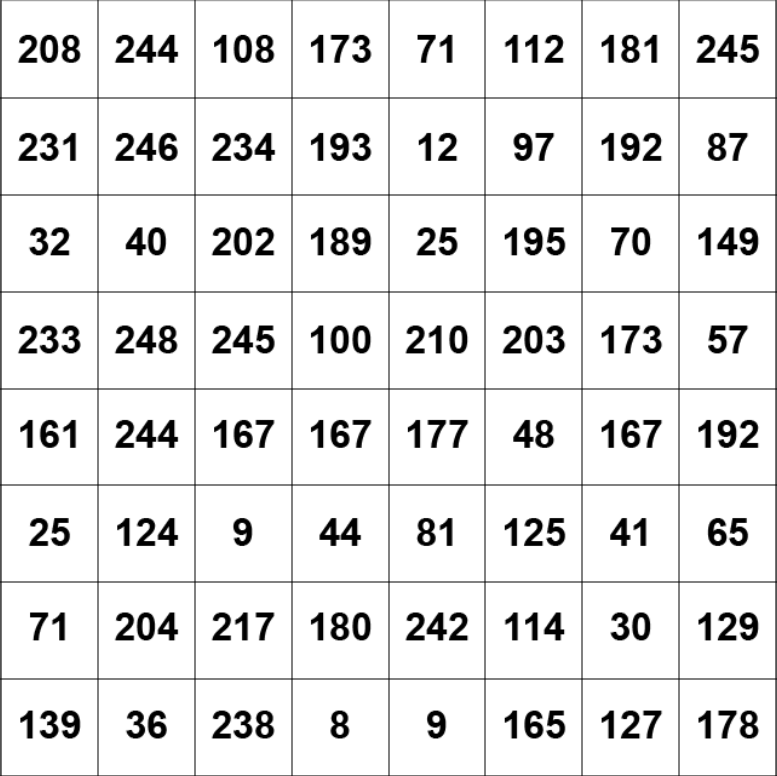
\includegraphics[width=.5\linewidth]{MatrizNivelCinza}
  \caption{}
  \label{exemplo:sfig1}
\end{subfigure}%
\end{figure}


\end{frame}
\begin{frame}
\frametitle{Espaços de cor}
\begin{itemize}
  \item Modelos de representação de cores.
  \item RGB e YCbCr.
  \item Ambos compostos de três canais.
\end{itemize}
\end{frame}

\begin{frame}
\frametitle{RGB}
\begin{itemize}
  \item Canais vermelho(R), verde(G) e azul(B).
  \item Matrizes contém fatores de influência de cada cor na imagem final.
\end{itemize}

	\begin{equation}
			C_{i,j} = p_{i,j,1} . R + p_{i,j,2} . G + p_{i,j,3} . B ,  (1<i<M, 1<j<N)
	\label{eq:corRGB}
	\end{equation}

\end{frame}

\begin{frame}
\frametitle{RGB}

\begin{figure}
  \centering
  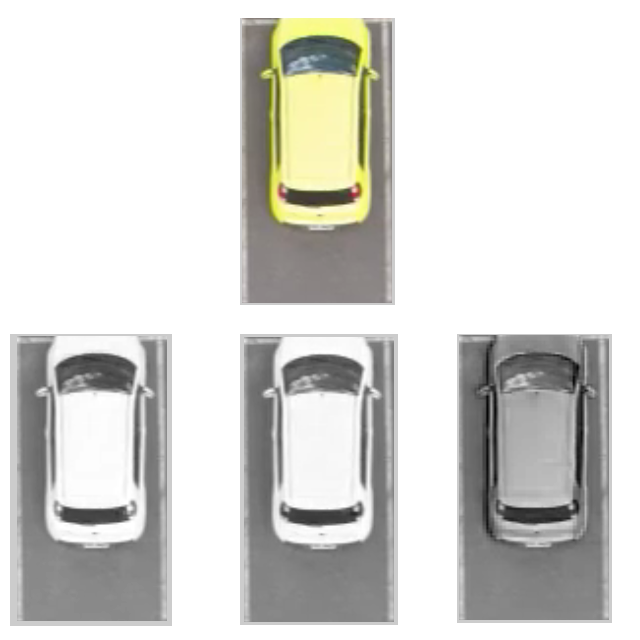
\includegraphics[width=.4\textwidth]{exemploRGBFinal}
  \caption{Uma imagem RGB e seus três canais separados.}
\end{figure}

\end{frame}

\begin{frame}
\frametitle{YCbCr}
\begin{itemize}
\item Usado em vídeos por sua capacidade de compressão.
\item Canais de luminância(Y), crominância azul(Cb) e crominância vermelha(Cr).
\item Pode ser obtida através da imagem RGB.
\item Canais de crominância são gerados pela diferença entre Y e canais R e B. 
\end{itemize}

\begin{equation}
	Y = 0,299.R + 0,587.G + 0,114.B
\label{eq:Y}
\end{equation}

\end{frame}

\begin{frame}
\frametitle{YCbCr}
\begin{figure}
 \centering
 \begin{subfigure}{.2\textwidth}
  \centering
  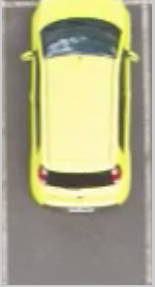
\includegraphics[width=.5\linewidth]{exemploRGB}
\end{subfigure}\
\begin{subfigure}{.2\textwidth}
  \centering
  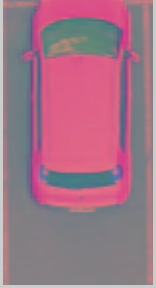
\includegraphics[width=.5\linewidth]{exemploycbcr}
\end{subfigure}
\end{figure}

\begin{figure}
  \centering
  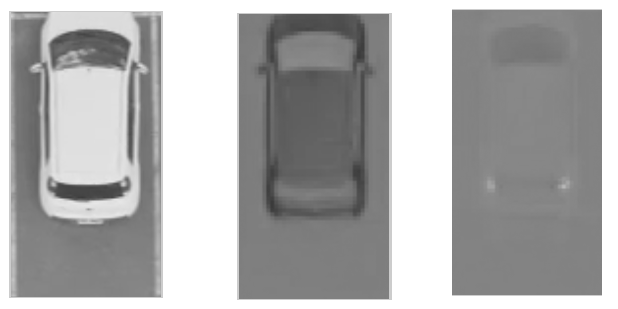
\includegraphics[width=.4\linewidth]{exemploYCbCrFinal}
  \caption{A imagem YCbCr obtida de uma imagem RGB e seus canais.}
\end{figure}
\end{frame}

\begin{frame}
\frametitle{Descritores de textura}
\begin{block}{}
Algoritmos que retorna valores que representam padrões de uma imagem analisada. Analisam a imagem como um todo, ao invés de \textit{pixel-a-pixel}.
\end{block}
\end{frame}

\begin{frame}
\frametitle{GLCM}
\begin{itemize}
\item \textit{Gray Level Co-ocurrence Matrix}.
\item Aplicada em imagens de nível de cinza.
\item Medidas estatísticas.
\item Analisa uma certa relação espacial entre dois \textit{pixels}.
\item Para este trabalho, a relação é a vizinhança direita.
\end{itemize}
\end{frame}

\begin{frame}
\frametitle{GLCM}
\begin{itemize}
\item Saída do algoritmo é uma matriz $MxM$ onde $M$ é o maior nível de cinza possível.
\end{itemize}

\begin{figure}
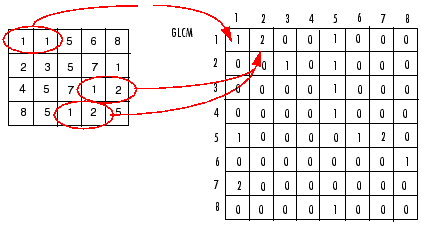
\includegraphics[width=7cm]{GLCM} 
\centering
\caption{Exemplo da elaboração da GLCM. Extraída de https://www.mathworks.com/help/images/ref/graycomatrix.html}
\label{fig:GLCM}
\end{figure}
\end{frame}

\begin{frame}
\frametitle{GLCM}
\begin{block}{Medidas}
\begin{itemize}
\centering
\item[Contraste:] $C = \sum_{i,j} (i-j)^{2}P_{(i,j)}$
\item[Correlação:] $Co = \sum_{i,j} \frac{(i - \mu_i)(j - \mu_j)P_{(i,j)}}{\sigma_i\sigma_j}$
\item[Energia:]$E = \sum_{i,j} P_{(i,j)}^{2}$
\item[Homogeneidade:]$H = \sum_{i,j} \frac{P_{(i,j)}}{1+|i-j|}$
\centering
\end{itemize}
\end{block}
\end{frame}

\begin{frame}
\frametitle{Vídeos}
\begin{block}{Vídeo}
Representação de cenas dinâmicas do mundo real. A sensação de movimento é criada através da exibição de imagens digitais a uma taxa adequada.
\end{block}

\begin{block}{Detecção de Movimento}
Análise da diferença entre dois quadros para estimar a movimentação de objetos na cena.
\end{block}
\end{frame}

\begin{frame}
\frametitle{Fluxo óptico}
\begin{itemize}
\item Estimativa da velocidade do movimento de cada \textit{pixel} da imagem.
\item $I(x,y,t) = I(x+dx, y+dy, t+dt)$
\item Restrição do Fluxo óptico: $\nabla Iv + I_t = 0$.
\item É preciso analisar a vizinhança para encontrar ambos os componentes de $v$.
\item Método Lucas-Kanade: vizinhança local.
\end{itemize}
\end{frame}

\begin{frame}
\frametitle{Fluxo óptico}
\begin{figure}
 \centering
\begin{subfigure}{.4\textwidth}
  \centering
  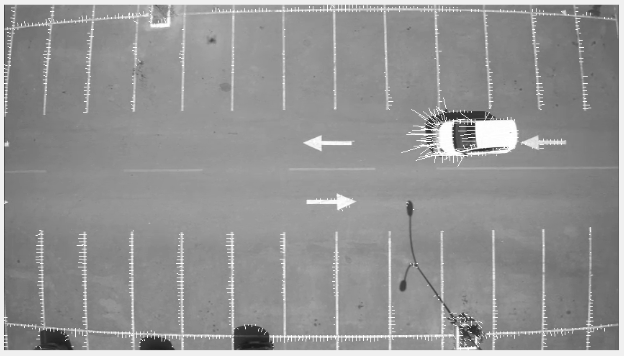
\includegraphics[width=.8\linewidth]{velocidadevetores}
	\caption{}
\end{subfigure}\
\begin{subfigure}{.4\textwidth}
  \centering
  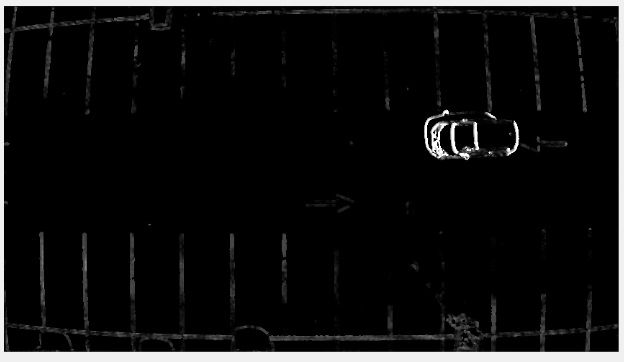
\includegraphics[width=.8\linewidth]{velocidademagnitude}
	\caption{}
\end{subfigure}
\caption{(a) Representação dos vetores de velocidade estimado pelo fluxo óptico. (b) Imagem em níveis de cinza onde a intensidade do \textit{pixel} representa a magnitude do seu vetor de velocidade.}
\end{figure}
\end{frame}

\section{Redes Neurais Artificiais}

\begin{frame}
\frametitle{Redes Neurais Artificias}
\begin{block}{Redes Neurais}
Sistemas inspirados no cérebro humano para realização de tarefas como classificação de padrões e ajuste de funções. Usam elementos de processamento distintos que trabalham paralelamente(neurônios).
\end{block}

\begin{block}{Haykin define como:}
 "...um processador distribuído massivamente paralelo composto por unidades simples de processamento, que possui uma propensidade natural a armazenar conhecimento experimental e torná-lo disponível para uso."
\end{block}
\end{frame}

\begin{frame}
\frametitle{Neurônio}
\begin{figure}
\centering
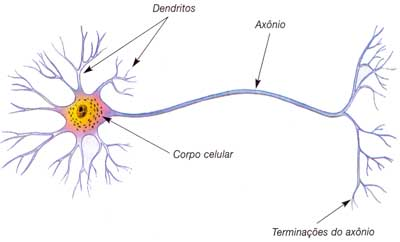
\includegraphics[width=.6\textwidth]{neuronio}
\caption{A estrutura básica de um neurônio humano}
\end{figure}
\end{frame}

\begin{frame}
\frametitle{Neurônio Artificial}
\begin{figure}
\centering
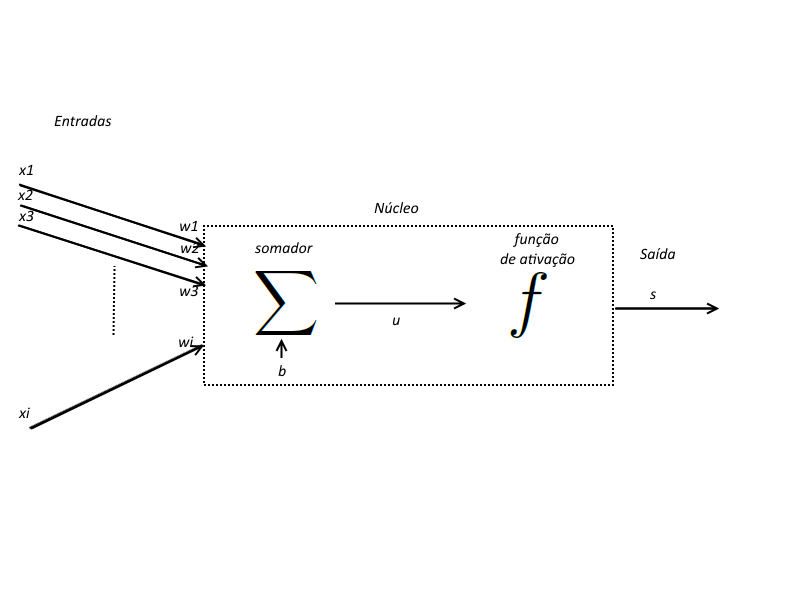
\includegraphics[width=.6\textwidth]{NeuronioArtificial}
\caption{A estrutura básica de um neurônio artificial}
\end{figure}
\end{frame}

\begin{frame}
\frametitle{Arquitetura \textit{Feed-forward}}
\begin{itemize}
\item Arquitetura para organização dos neurônios de uma rede neural artificial.
\item Camada de entrada, camadas ocultas e camada de saída.
\item Informação flui apenas no sentido entrada-saída.
\item Cada neurônio de uma camada é ligado a todos da camada seguinte.
\item Não há ligação entre neurônios de uma mesma camada.
\end{itemize}
\end{frame}

\begin{frame}
\frametitle{Arquitetura \textit{Feed-forward}}
\begin{figure}
\centering
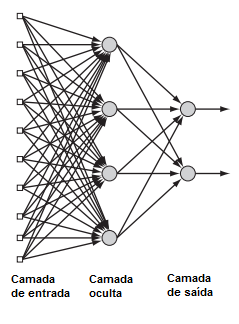
\includegraphics[width=.3\textwidth]{feedforward}
\caption{A arquitetura feed-forward. Adaptada de \cite{Haykin}}
\end{figure}
\end{frame}

\begin{frame}
\frametitle{Treinamento}
\begin{itemize}
\item Processo onde a rede é configurada para realizar a tarefa específica para qual foi criada.
\item Aprendizado: capacidade da rede de aproximar o comportamento das entradas durante o treinamento.
\item Generalização: capacidade da rede de prever e operar sobre entradas que não estavam no conjunto de treinamento.
\item Valores dos pesos $w$ e dos deslocamentos $b$ são definidos.
\end{itemize}
\end{frame}

\begin{frame}
\frametitle{Treinamento}
\begin{itemize}
\item \textbf{Conjunto de treinamento:} Conjunto utilizado para a calibração dos valores de $w$ e $b$.
\item \textbf{Conjunto de validação:} Após cada iteração do treinamento, a rede valida os valores configurados usando este conjunto.
\item \textbf{Conjunto de testes:} A rede é apresentada a este conjunto ao final do treinamento para verificação do funcionamento.
\end{itemize}
\end{frame}

\begin{frame}
\frametitle{Treinamento}
\begin{block}{Treinamento Supervisionado}
Elementos dos conjuntos de treinamento e validação são as entradas e os gabaritos da saídas desejadas de cada entrada. Treina até que a saída seja suficientemente próxima do gabarito.
\end{block}

\begin{block}{Treinamento Não-Supervisionado}
A rede recebe um conjunto de entradas e aprende características intrínsecas dos dados apresentados.
\end{block}

\end{frame}

\begin{frame}
\frametitle{Classificação de padrões}
\begin{itemize}
\item Consiste em analisar padrões de um conjunto de dados e designar o conjunto a uma classe pré-determinada.
\item A rede analisa características ou \textit{features}.
\item \textit{Features} devem ser descritivos e discriminantes.
\item Limiar de decisão.
\item A rede determina a probabilidade de que uma entrada pertença a uma classe.
\end{itemize}
\end{frame}

\begin{frame}
\frametitle{Classificação de padrões}
\begin{figure}
\centering
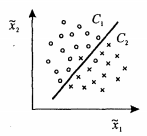
\includegraphics[width=5cm]{features}
\label{fig:features}
\caption{Um gráfico que mostra duas características $\tilde{x}_1$ e $\tilde{x}_2$ de um problema de classificação hipotético. Extraída de \cite{NNForPR}.}
\end{figure}
\end{frame}


\section{Solução proposta}

\begin{frame}
\frametitle{Fluxograma}
\begin{figure}
	\centering
	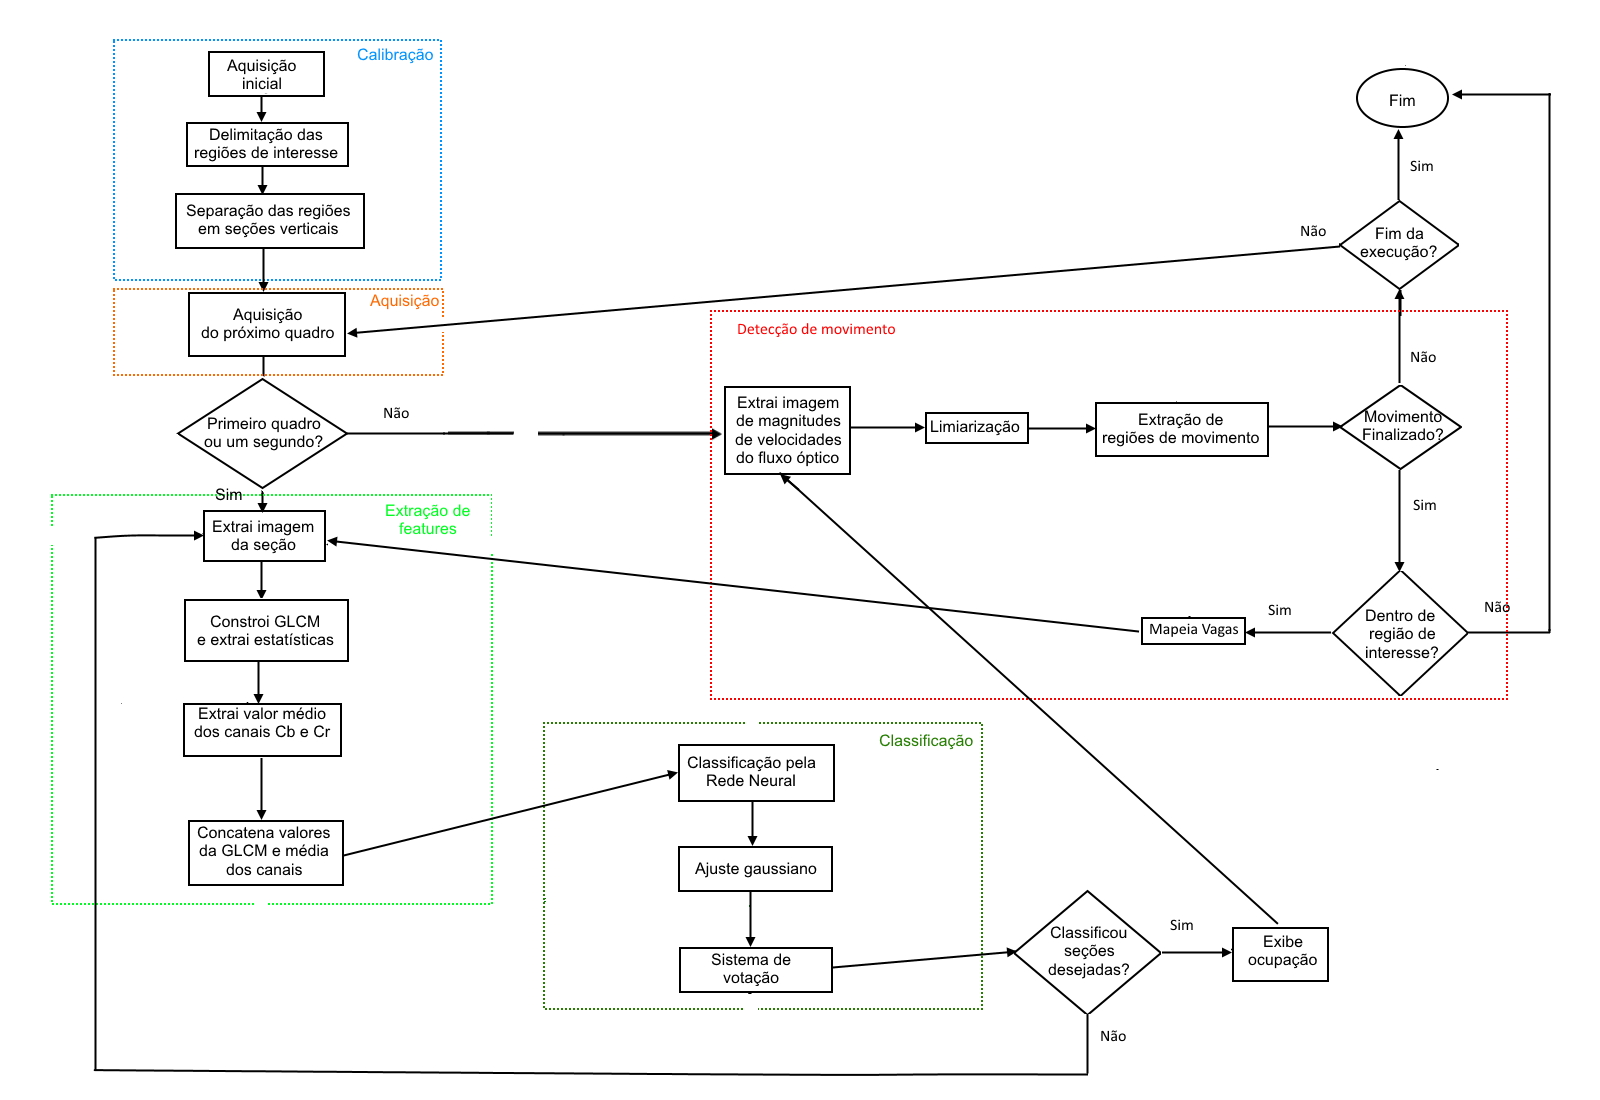
\includegraphics[width=1\textwidth, height=.8\textheight]{fluxograma}
	\centering
\end{figure}
\end{frame}

\begin{frame}
\frametitle{Aquisição}
    \begin{block}{}
    Imagens de câmeras montadas em postes de luz ou similar.
    \end{block}
\begin{figure}
	\centering
	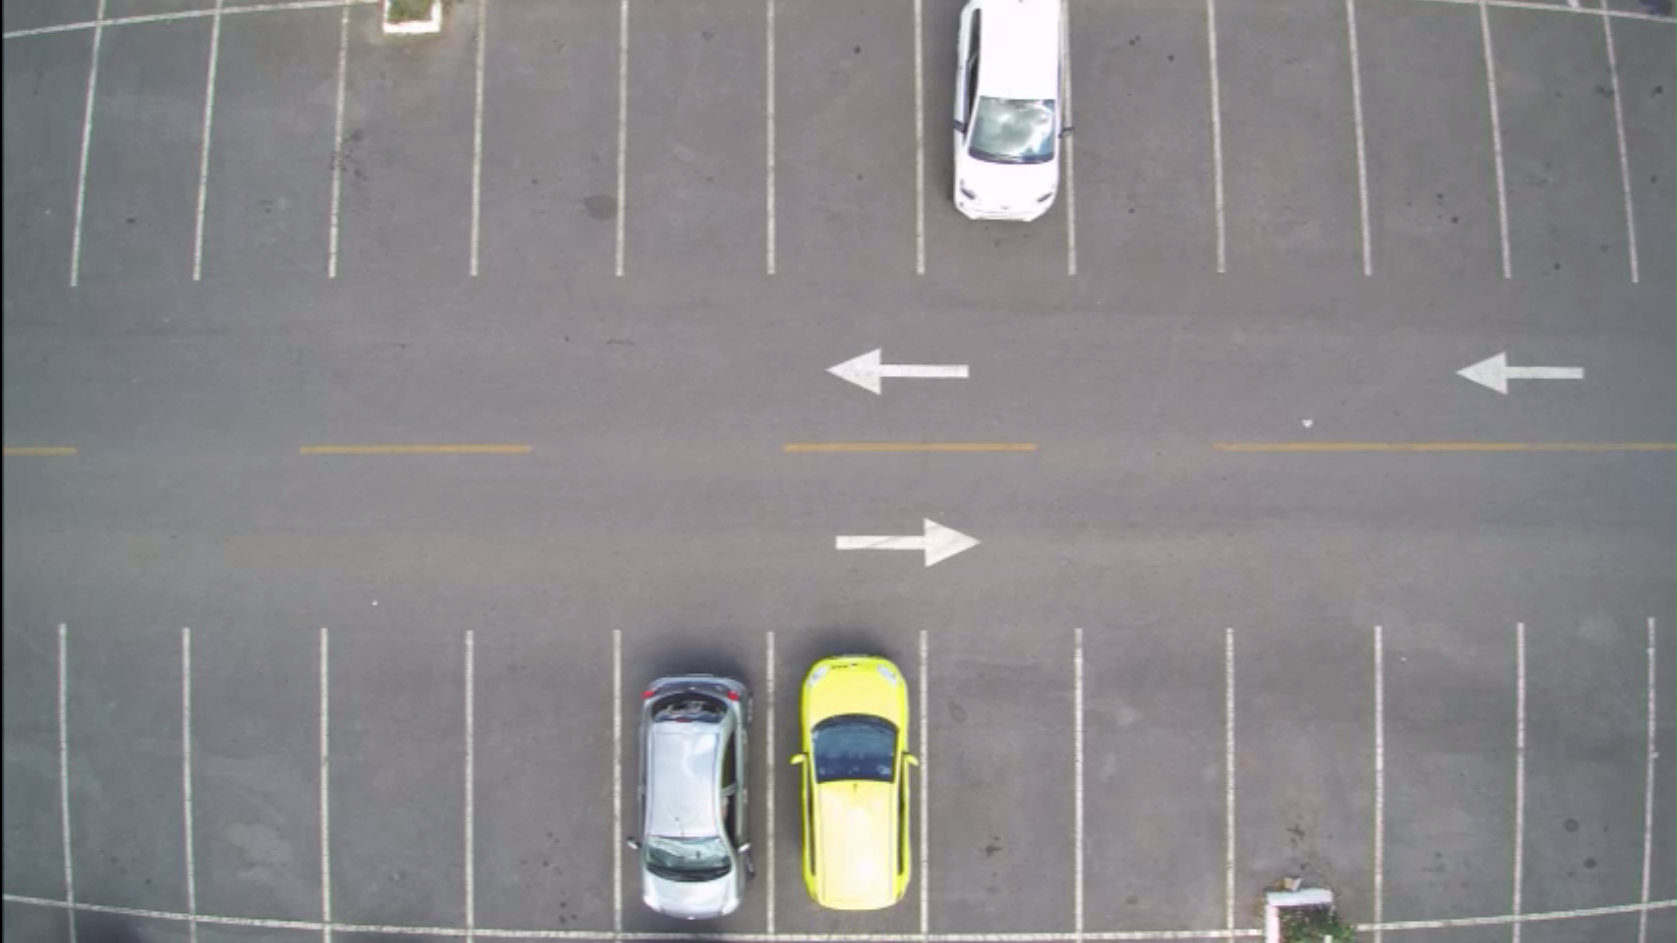
\includegraphics[width=.4\textwidth]{Vazio3}
	\centering
\end{figure}
\end{frame}

\begin{frame}
\frametitle{Regiões de interesse}
\begin{block}{}
\begin{itemize}
\item Definidas no momento de instalação.
\item Não devem ter intersecção.
\item Regiões onde há vagas na imagem.
\end{itemize} 
\end{block}
\begin{figure}
	\centering
	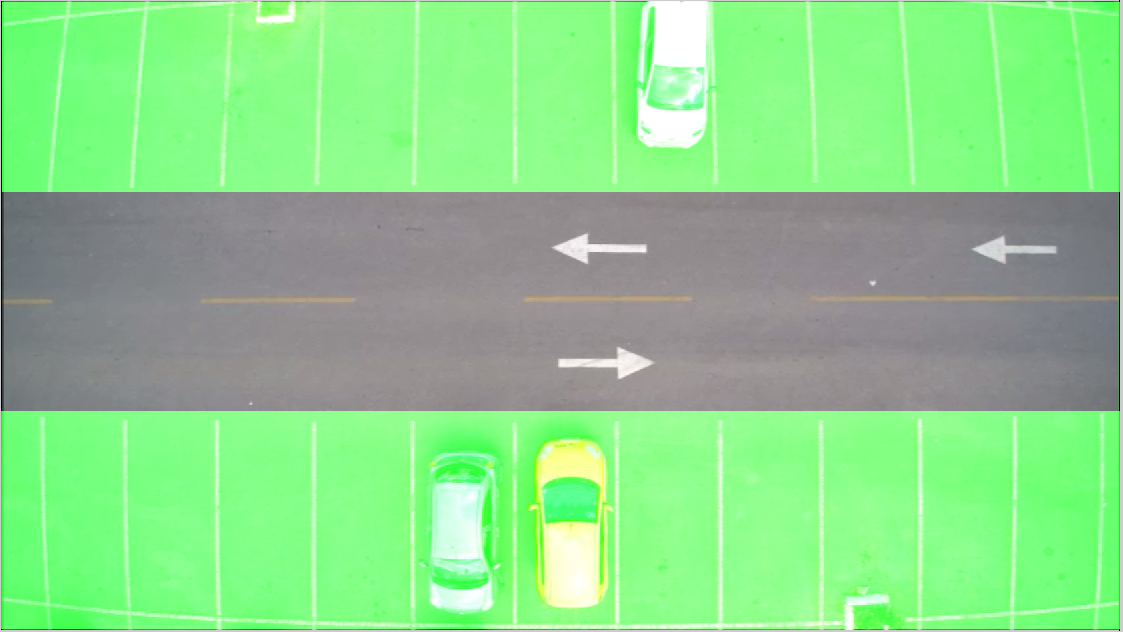
\includegraphics[width=.4\textwidth]{ROIs}
	\centering
\end{figure}
\end{frame}

\begin{frame}
\frametitle{Seções verticais}
\begin{block}{}
Cada ROI é dividida em um número igual de seções verticais.
\end{block}
\begin{figure}
	\centering
	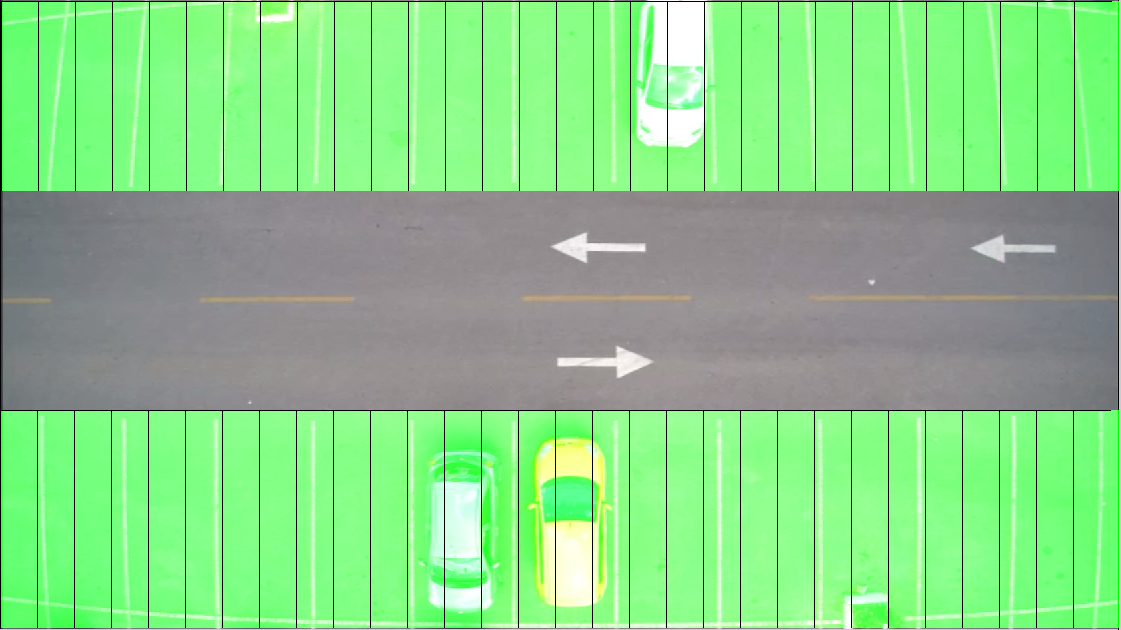
\includegraphics[width=.4\textwidth]{Secoes}
	\centering
\end{figure}

\end{frame}

\begin{frame}
\frametitle{Classificação das seções}
	A classificação tem 4 etapas:
   \begin{itemize}
      \item Extração das características.
      \item Classificação pela Rede Neural.
      \item Ajuste pelos vizinhos.
      \item Sistema de votação
    \end{itemize}
\end{frame}

\begin{frame}
\frametitle{Extração das características}
Imagens individuais de cada seção são extraídas.
\begin{figure}
	\centering
	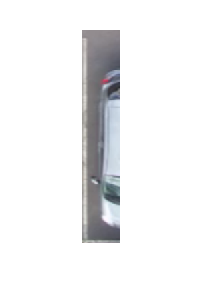
\includegraphics[width=.4\textwidth]{imgSecao}
	\centering
\end{figure}
\end{frame}

\begin{frame}
\frametitle{Extração das características}
\begin{itemize}
\item Medidas GLCM: $\begin{pmatrix}
	Contraste\\Correlação\\Energia\\Homogeneidade
	\end{pmatrix}$
\item Médias dos canais de crominância: $\begin{pmatrix}
	MCb\\MCr
	\end{pmatrix}$
\item Vetor final de entrada: $\begin{pmatrix}
	Contraste\\Correlação\\Energia\\Homogeneidade\\MCb\\MCr
	\end{pmatrix}$
\end{itemize}

\end{frame}

\begin{frame}
\frametitle{Classificação da Rede Neural Artificial}
   \begin{itemize}
   \item Duas classes possíveis: carro(1) ou vaga (2).
   \item Rede neural recebe vetor de entrada e retorna vetor com probabilidade de cada classe.
   \end{itemize}
  \begin{equation}
	\centering	
	\begin{pmatrix}
	P_1\\P_2
	\end{pmatrix}  
	\centering
  \end{equation}

\end{frame}

\begin{frame}
\frametitle{Ajuste dos vizinhos}

A classe das seções vizinhas influência a classificação de uma seção de acordo com as equações:

   \begin{equation}
	f(s,v) = \frac{1}{\sqrt{2\pi\sigma^2}} \exp^{\frac{-(i_s-i_v)^2}{2\sigma^2}} 
	\end{equation}

\begin{equation}
	P_{cv}  = P_{cv}(1+f(s,v))
\end{equation}

\begin{equation}
	P_{\overline{cv}}  = P_{\overline{cv}}(1-f(s,v))
\end{equation}
\end{frame}

\begin{frame}
\frametitle{Ajuste dos Vizinhos}
  \begin{figure}
	\centering
	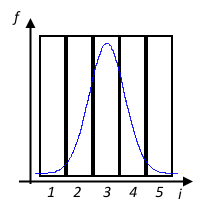
\includegraphics[width=.4\textwidth]{Influencia}
	\centering
\end{figure}
\end{frame}

\begin{frame}
\frametitle{Ajuste dos Vizinhos}
  Ajuda a evitar erros como este:
  \begin{figure}
	\centering
	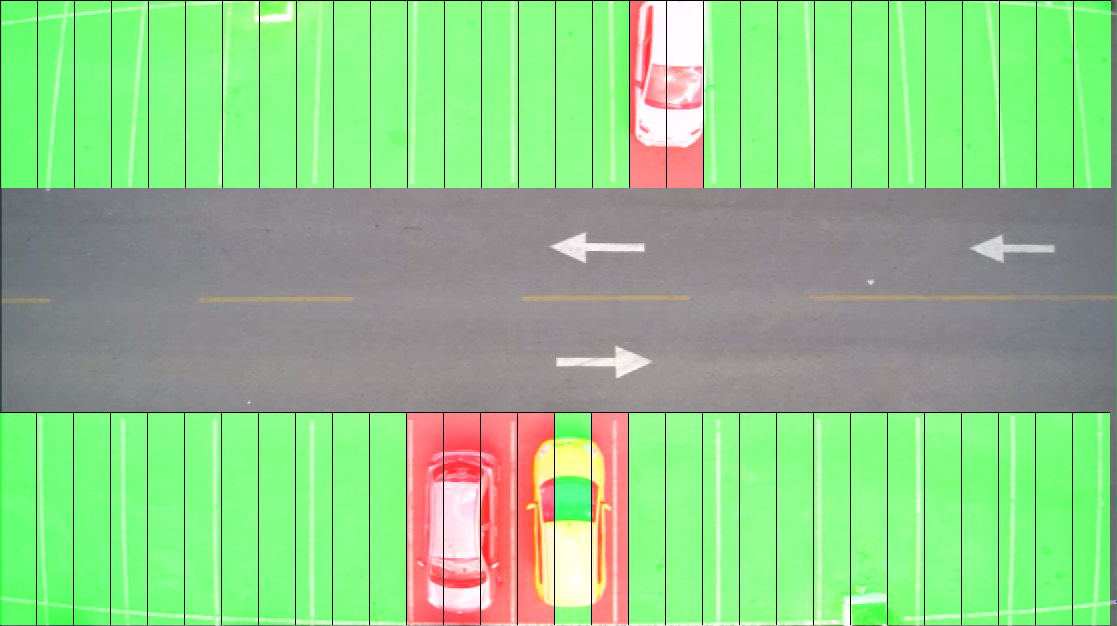
\includegraphics[width=.4\textwidth]{erroMeio}
	\centering
\end{figure}
\end{frame}

\begin{frame}
\frametitle{Sistema de votação}
\begin{itemize}
\item Votação define se a seção está estabilizada ou não.
\item Voto é baseado no vetor de probabilidades modificado pelo ajuste dos vizinhos.
\item $voto= 
\begin{cases}
    1,& \text{se } P_1 >= 0,6\\
    2,& \text{caso contrário}
\end{cases}$.
\item Seção não muda de classe se estiver estabilizada.
\item Evitar flutuações na ocupação das seções.
\end{itemize}
\end{frame}

\begin{frame}
\frametitle{Sistema de votação}
  \begin{figure}
	\centering
	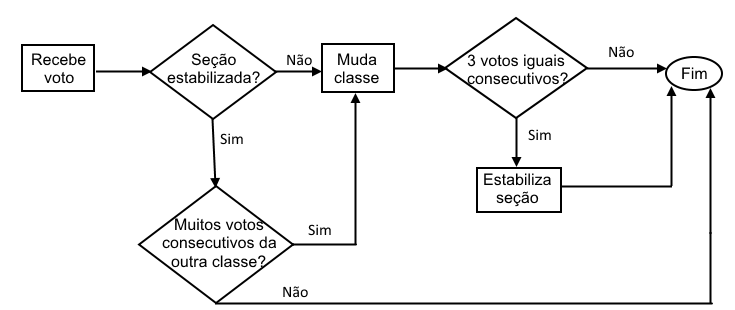
\includegraphics[width=.8\textwidth]{fluxogramaVotos}
	\centering
\end{figure}

\end{frame}

\begin{frame}
\frametitle{Seções classificadas}
  \begin{figure}
	\centering
	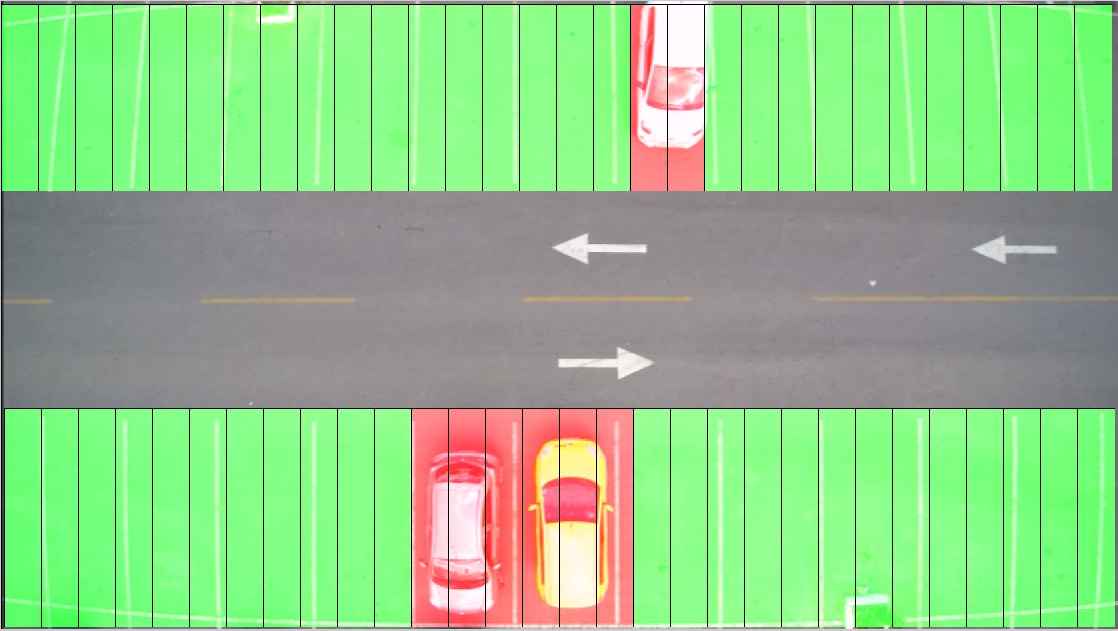
\includegraphics[width=.8\textwidth]{Classificada}
	\centering
\end{figure}
\end{frame}

\begin{frame}
\frametitle{Detecção de movimento}
\begin{itemize}
\item Movimento detectado pelo método do Fluxo Óptico
\item Resultado: imagem que representa as magnitudes dos vetores velocidade
\item Essa imagem é limiarizada para eliminar os vetores não significativos.
\end{itemize}
\end{frame}

\begin{frame}
\frametitle{Detecção de movimento}
\begin{figure}
\centering
\begin{subfigure}{.5\textwidth}
  \centering
  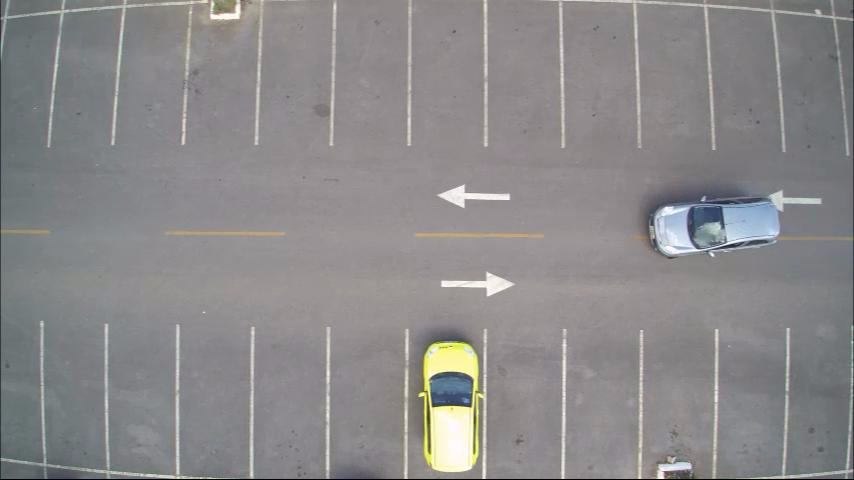
\includegraphics[width=.8\linewidth]{quadroMov}
\end{subfigure}%
\begin{subfigure}{.5\textwidth}
  \centering
  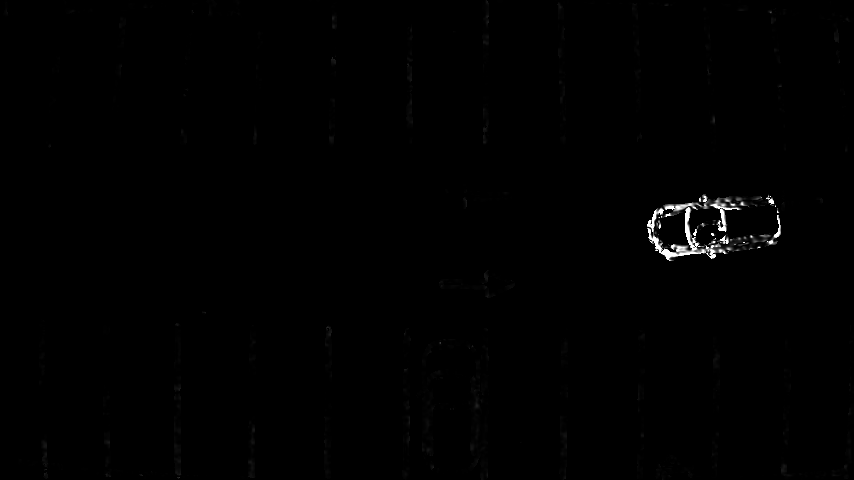
\includegraphics[width=.8\linewidth]{mags}
\end{subfigure}\\
\begin{subfigure}{.5\textwidth}
  \centering
  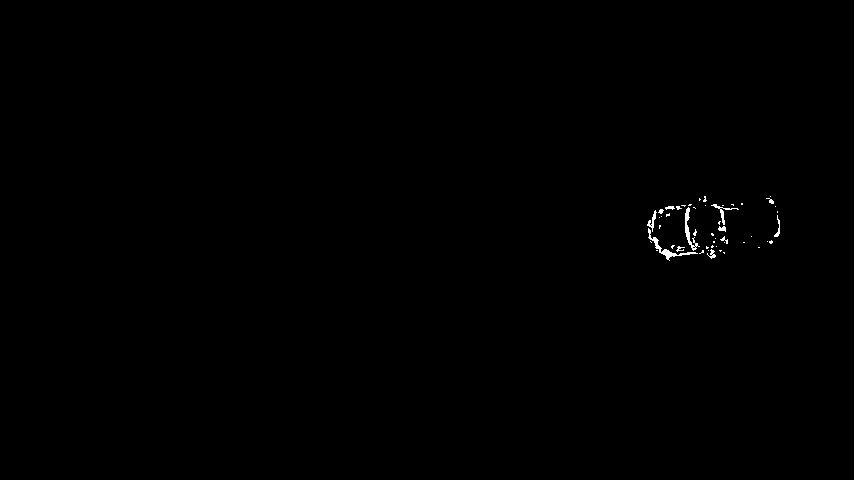
\includegraphics[width=.8\linewidth]{limiarizada}
\end{subfigure}
\centering
\end{figure}
\end{frame}

\begin{frame}
\frametitle{Regiões do movimento}
\begin{block}{}
Regiões são detectadas através de análise dos pixels brancos da imagem limiarizada.
\end{block}

\begin{figure}
\centering
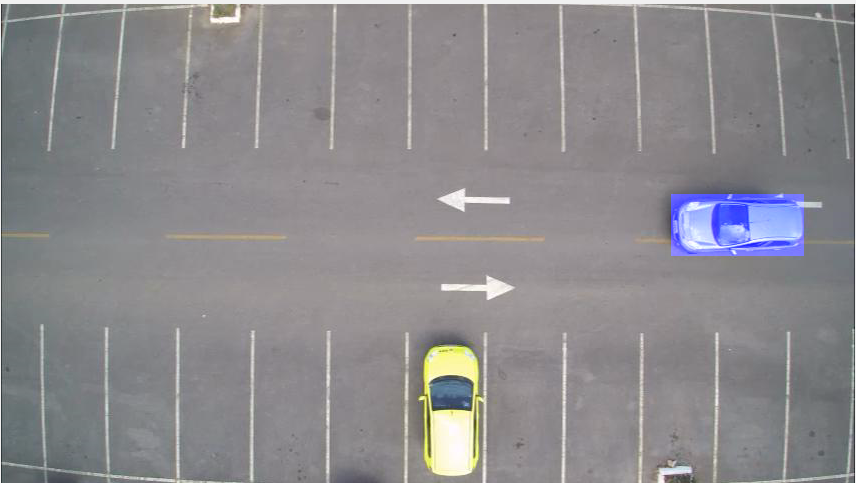
\includegraphics[width=.4\textwidth]{retanguloMovimento}
\centering
\end{figure}
\end{frame}

\begin{frame}
\frametitle{Mapeamento das vagas}
\begin{itemize}
\item No momento inicial da execução conjuntos de seções ocupadas consecutivas formam uma vaga.
\item Quando um movimento termina, a posição aonde ele acabou e começou é analisada.
\item As seções verticais interceptadas pelo movimento nestas posições ficam não-estabilizadas, são reclassificadas e marcadas como uma vaga.
\item Assume-se que os carros estão parando em vagas corretamente.
\end{itemize}
\end{frame}

\begin{frame}
\frametitle{Tratamento de intersecção de vagas}
\begin{block}{Modo simples}
Seções marcadas pelo movimento passam a fazer parte de uma vaga nova, vaga antiga é composta das seções restantes.
\end{block}

\begin{figure}
\centering
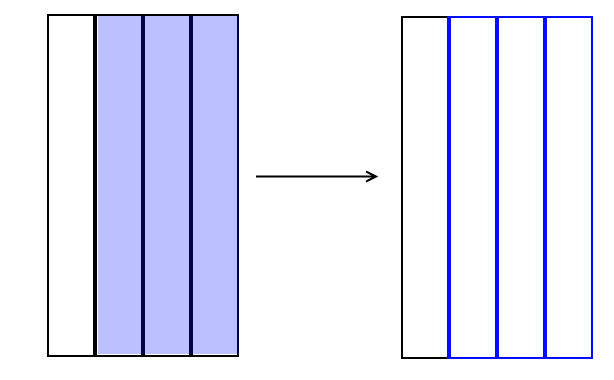
\includegraphics[width=.4\textwidth]{umasecao}
\centering
\end{figure}

\end{frame}

\begin{frame}
\frametitle{Tratamento de intersecção de vagas}
\begin{block}{Modo Complexo}
Segue um conjunto mais elaborado de regras:
\begin{itemize}
\item $S_m \supseteq V \Rightarrow V = S_m$
\item $S_m \subset V \Rightarrow V = S_m$. Caso $S_m - V$ seja um conjunto contínuo de um número suficiente de seções, uma nova vaga $V_2$ também é criada.
\item Se $S_m \cap V \neq \emptyset$ as seções da intereseção são divididas entre as duas vagas, dando preferência para $S_m$.  
\end{itemize}
\end{block}
\end{frame}

\section{Resultados Experimentais}
\begin{frame}
\frametitle{Aquisição dos vídeos}
Drone \textit{Yuneec Typhoon Q500+}.
\begin{figure}
\centering
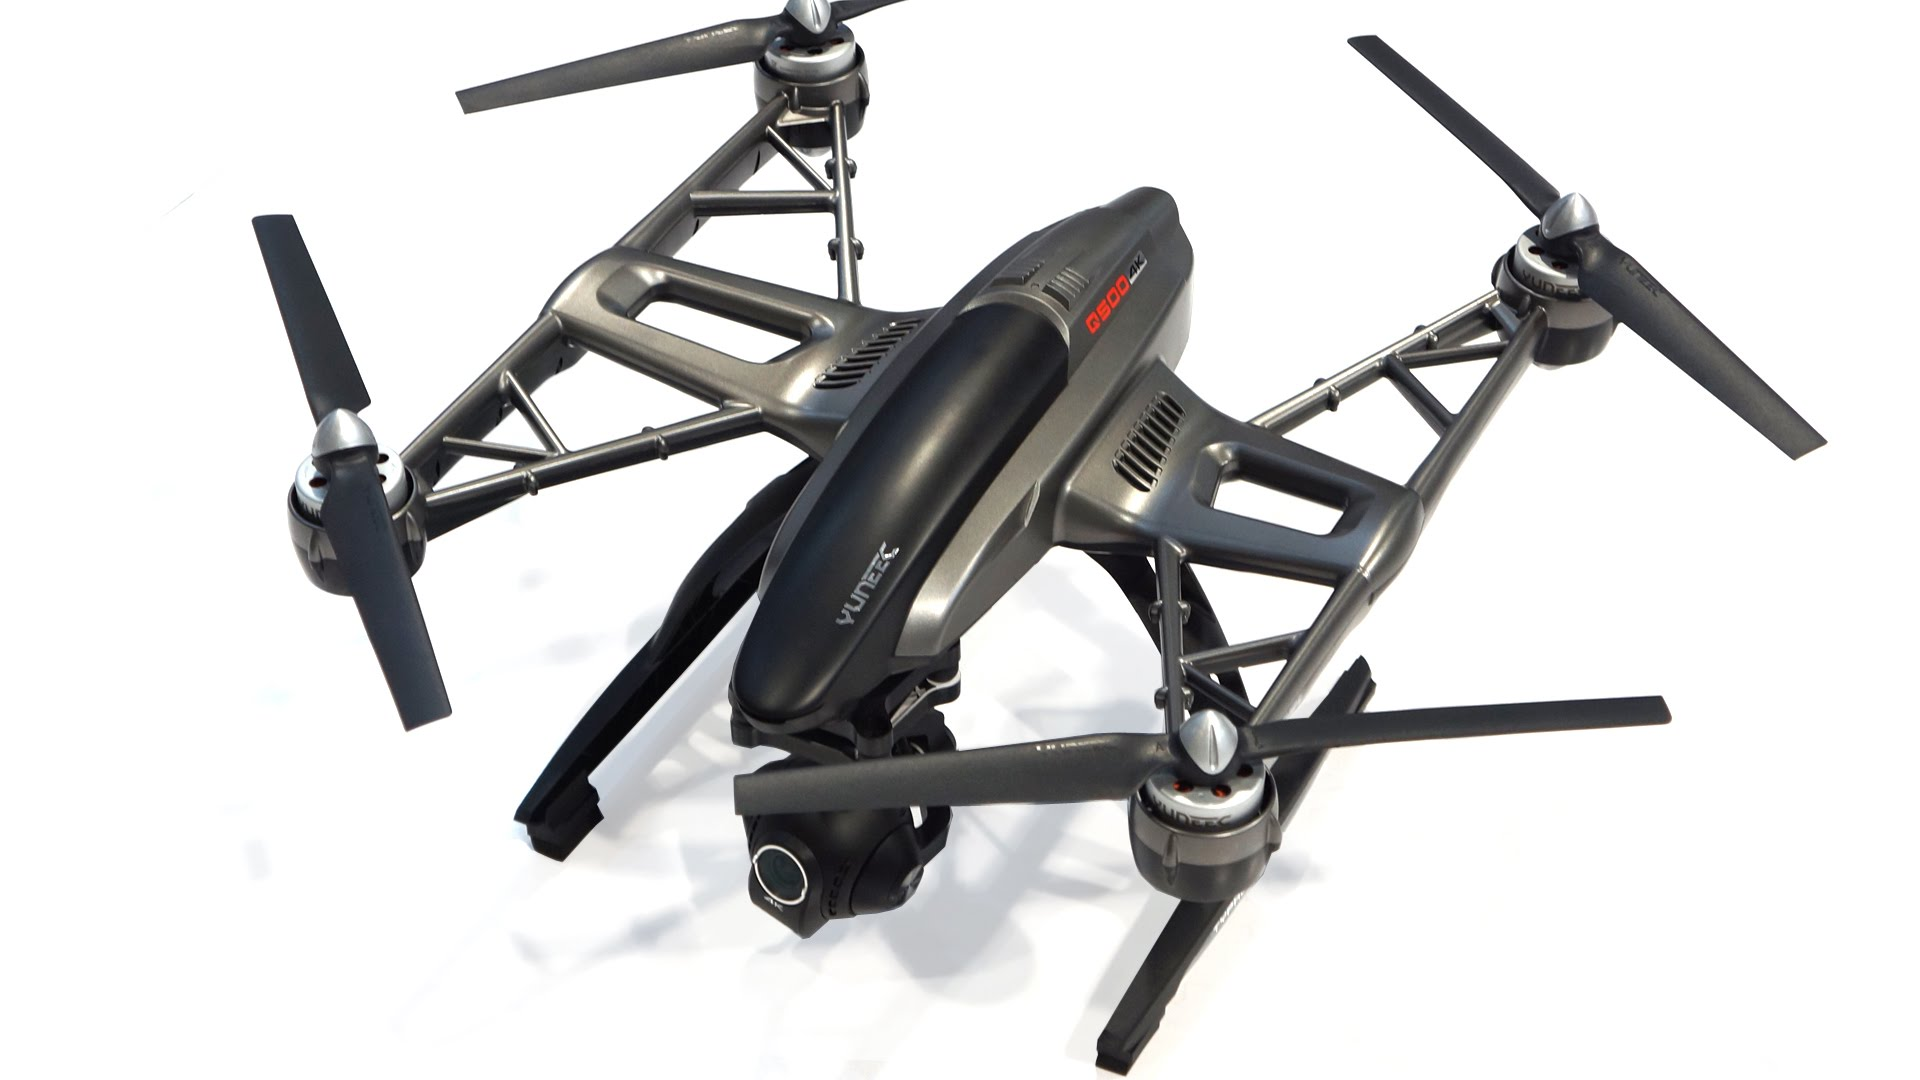
\includegraphics[width=8cm]{drone}
\cente
ring
\end{figure}
\end{frame}

\begin{frame}
\frametitle{Experimentos}
\begin{itemize}
\item Oito vídeos curtos com ROIs determinadas previamente divididas em $30$ seções verticais.
\item Desempenho do programa foi comparado com resultados de três observadores humanos: F, M e P.
\end{itemize}

\begin{figure}
\centering
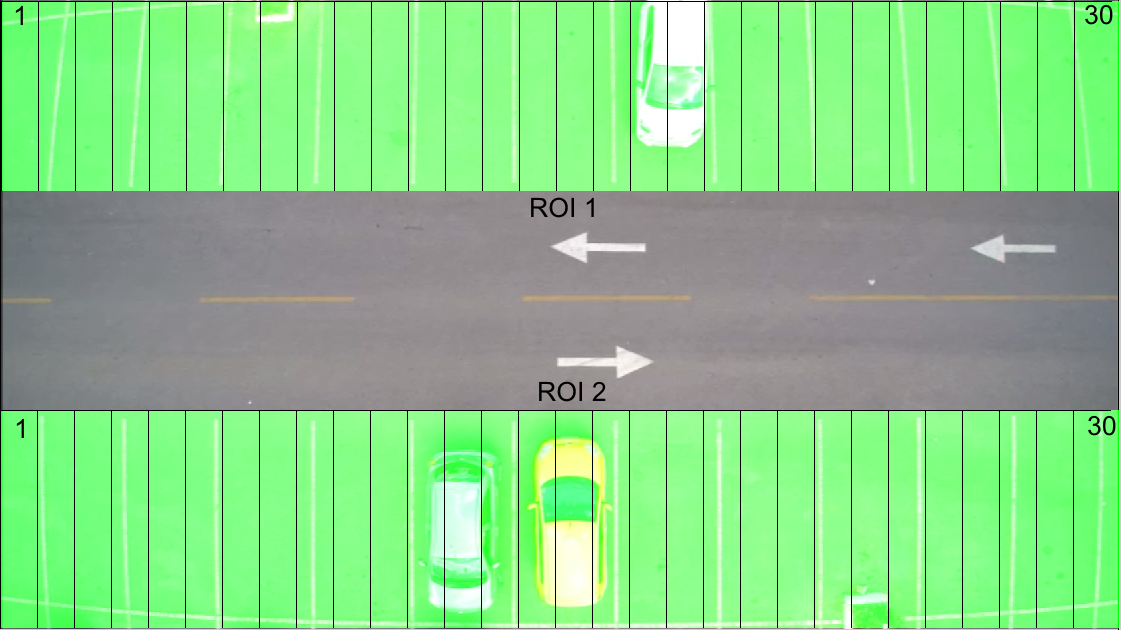
\includegraphics[width=4cm]{instrucoes}
\centering
\end{figure}
\end{frame}

\begin{frame}
\frametitle{Instruções}
Cada observador recebeu as seguintes instruções:
\begin{itemize}
  \item As regiões de interesse e as seções são numeradas como indicado na figura.
	\item Uma seção ocupada é aquela cuja maior parte de sua área está ocupada por um veículo.
	\item No momento inicial do vídeo ($0$ segundos), indique quais seções verticais estão ocupadas através do número das ROI e das seções, as outras serão assumidas como livres. Indique também o número de vagas ocupadas.
	\item Se a qualquer momento o estado de ocupação de uma seção mudar, indique o tempo da mudança, a seção onde ocorreu a mudança e a natureza da mudança(ocupada ou liberada).
\end{itemize}
\end{frame}

\begin{frame}
\frametitle{Experimentos}
\begin{block}{Ocupação das seções}
\begin{itemize}
\item Um acerto ocorre se em um determinado momento $t$, o programa e o observador concordam quanto a ocupação da seção.
\item $60$ acertos possíveis por segundo.
\item Taxa de acerto = número total de acertos/acertos possíveis.
\end{itemize}
\end{block}

\begin{block}{Vagas ocupadas}
\begin{itemize}
\item Um acerto ocorre se em um determinado momento $t$, o programa e o observador concordam quanto ao número de vagas ocupadas.
\item Número de acertos possíveis é igual a duração do vídeo.
\item Taxa de acerto = número total de acertos/acertos possíveis.
\end{itemize}
\end{block}
\end{frame}

\begin{frame}
\frametitle{Vídeo 1}

No primeiro caso de testes, o vídeo começa com um estacionamento vazio. Depois de alguns segundos um único veículo de cor branca entra na cena pela direita e estaciona em uma vaga na parte inferior da imagem. O vídeo tem $15s$ de duração.

\begin{figure}
\centering
\begin{subfigure}{.5\textwidth}
\centering
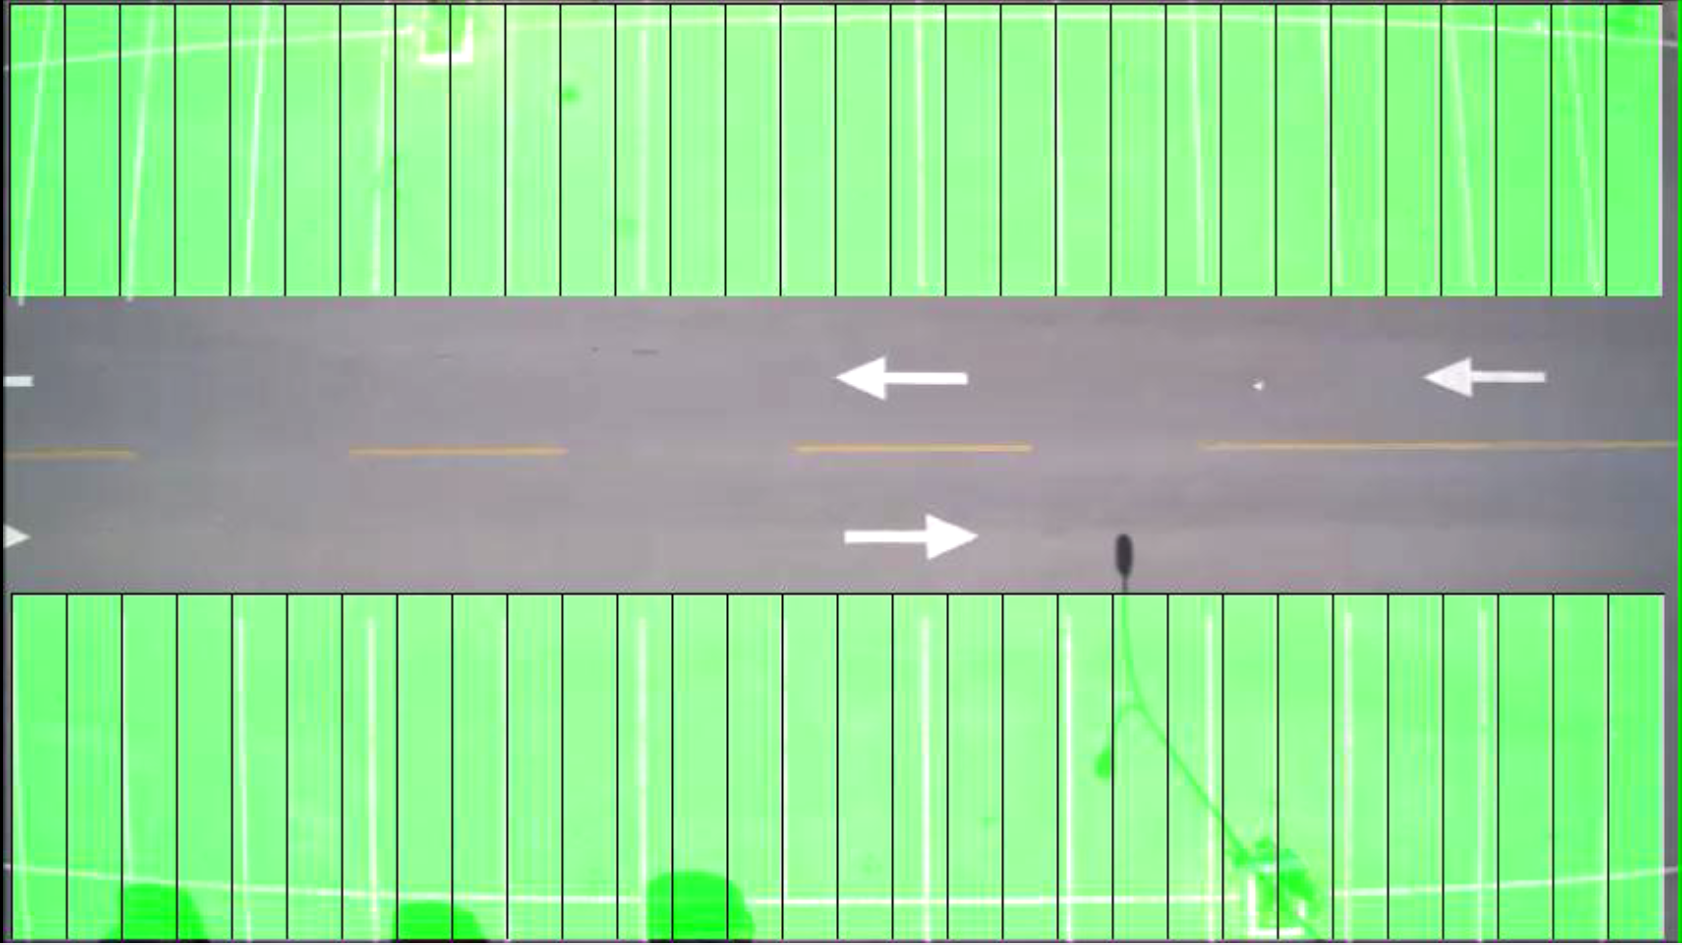
\includegraphics[width=.5\linewidth]{Video1Inicio}
\end{subfigure}\
\begin{subfigure}{.5\textwidth}
\centering
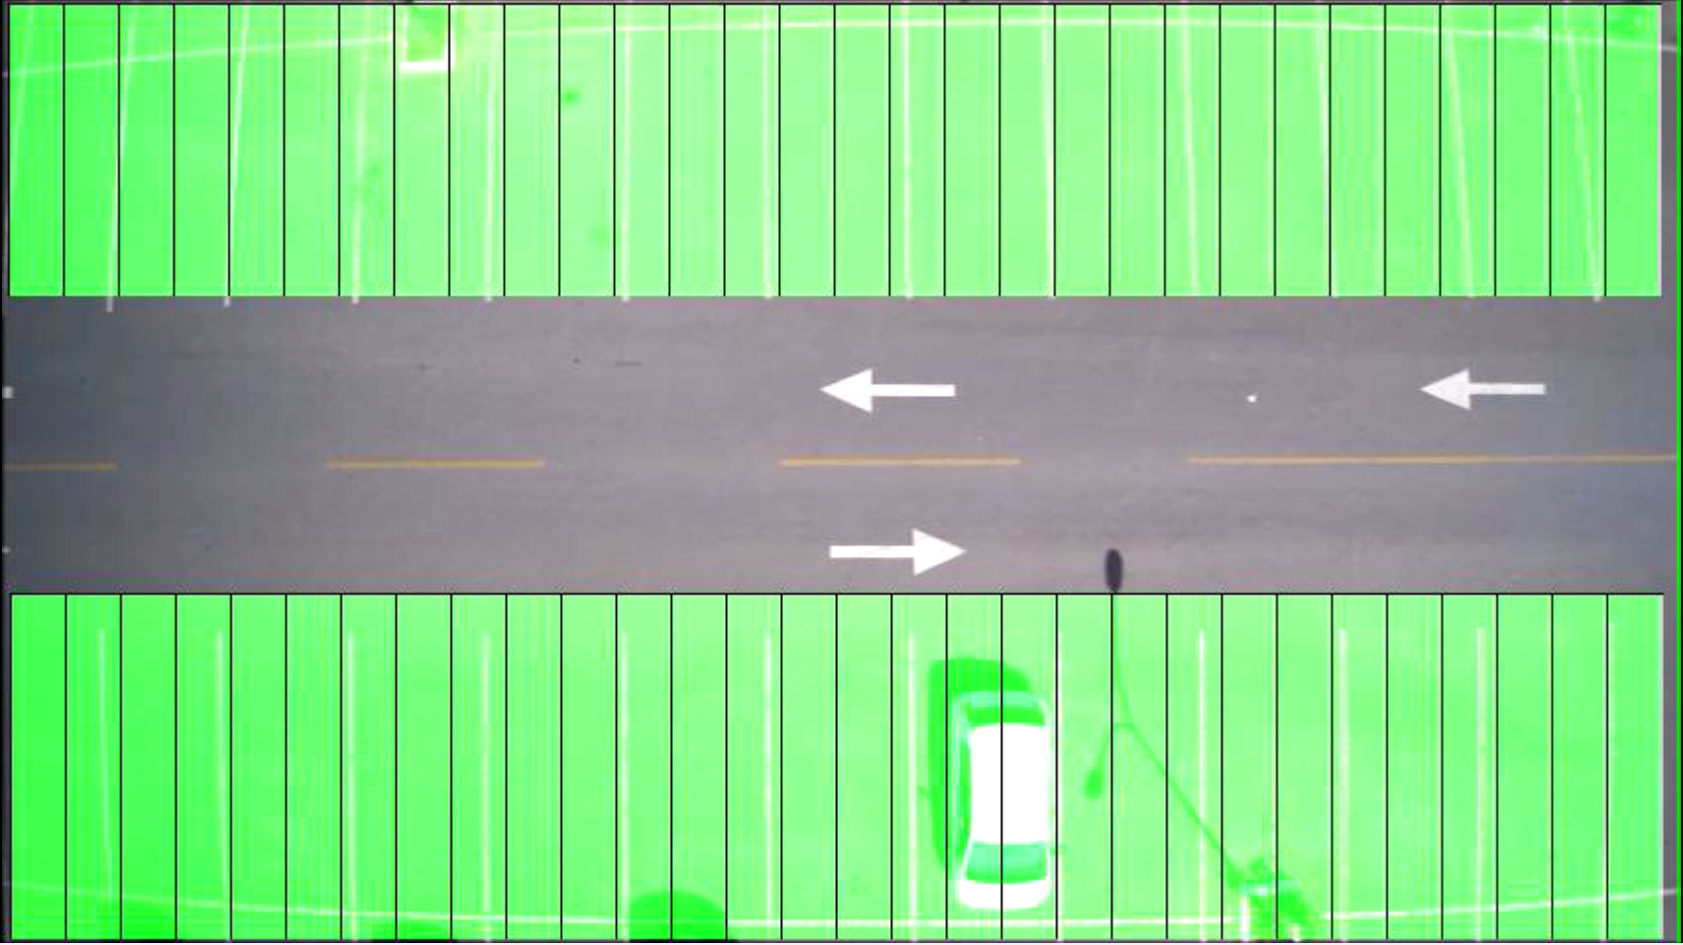
\includegraphics[width=.5\linewidth]{Video1Fim}
\end{subfigure}
\centering
\end{figure}	
\end{frame}

\begin{frame}
	\frametitle{Vídeo 1}
	
	\begin{center}
\begin{tabular}{|c||c||c|}
\hline
\multicolumn{3}{|c|}{Acertos - seções}  \\ \hline \hline
Observador & Acertos& Taxa de acertos \\ \hline
F & 886 & 98,44\% \\  \hline
P & 886 & 98,44\% \\ \hline
M & 884 & 98,22\% \\ \hline
Média & 885,3 & 98,37\% \\
\hline
\end{tabular}
\end{center}
\end{frame}

\begin{frame}
\frametitle{Vídeo 1}
\begin{center}
\begin{tabular}{|c||c||c|}
\hline
\multicolumn{3}{|c|}{Acertos - vagas}  \\ \hline \hline
Observador & Acertos & Taxa de acertos \\ \hline
F & 1 & 7\% \\  \hline
P & 1 & 7\% \\ \hline
M & 1 & 7\% \\ \hline
Média & 1 & 7\% \\
\hline
\end{tabular}
\end{center}
\end{frame}

\begin{frame}
\frametitle{Vídeo 2}

Neste vídeo, um carro branco está estacionado no conjunto inferior de vagas. Um veículo cinza entra pela direita e estaciona no conjunto superior de vagas. O vídeo tem uma duração de $10s$.

\begin{figure}
\centering
\begin{subfigure}{.5\textwidth}
\centering
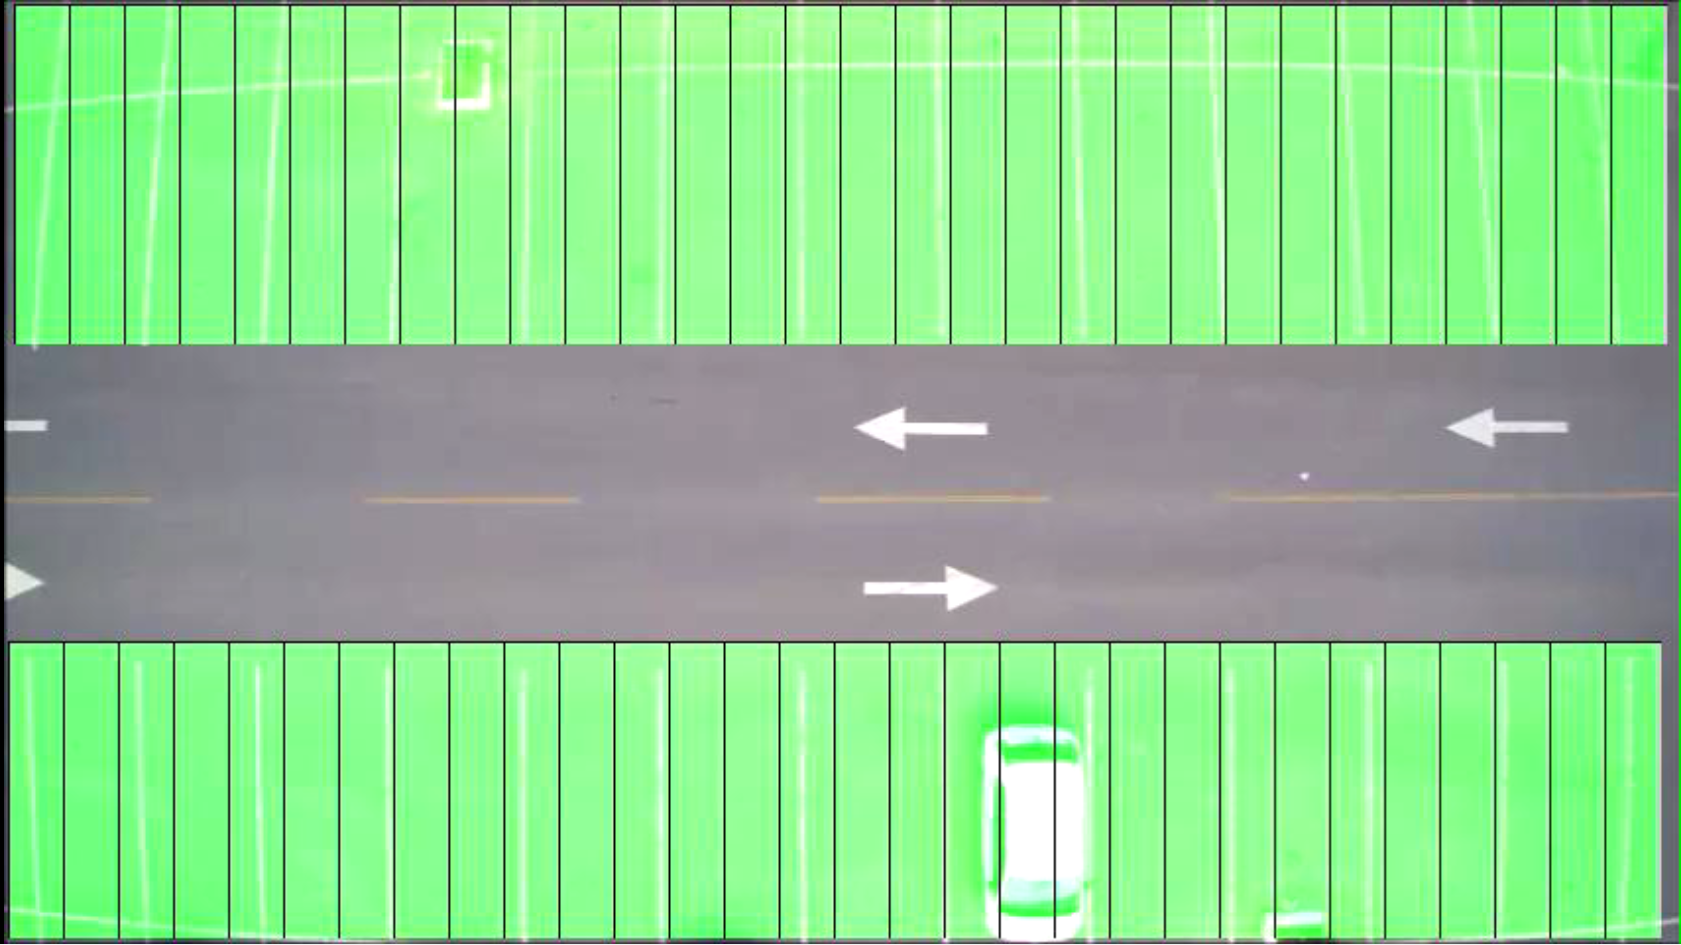
\includegraphics[width=.5\linewidth]{Video2Inicio}
\end{subfigure}\
\begin{subfigure}{.5\textwidth}
\centering
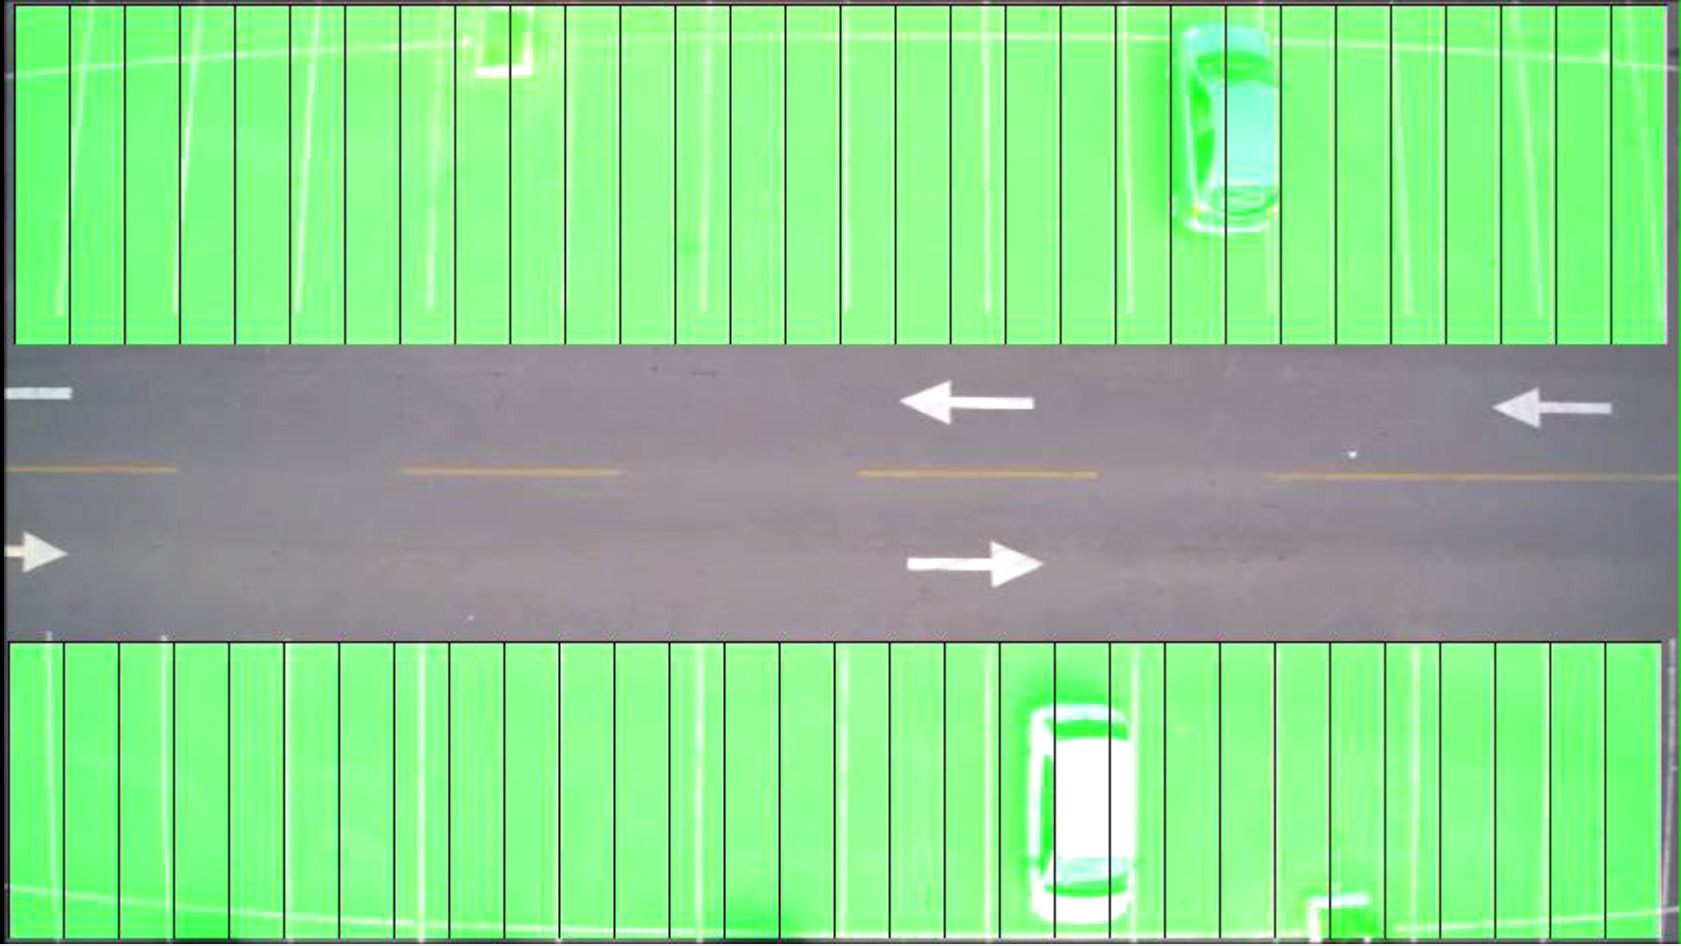
\includegraphics[width=.5\linewidth]{Video2Fim}
\end{subfigure}
\centering
\end{figure}	
\end{frame}

\begin{frame}
	\frametitle{Vídeo 2}
	
\begin{center}
\begin{tabular}{|c||c||c|}
\hline
\multicolumn{3}{|c|}{Acertos - seções}  \\ \hline \hline
Observador & Acertos & Taxa de acertos \\ \hline
F & 586 & 97,66\% \\  \hline
P & 586 & 97,66\% \\ \hline
M & 586 & 97,66\% \\ \hline
Média & 586 & 97,66\% \\
\hline
\end{tabular}
\end{center}
\end{frame}

\begin{frame}
\frametitle{Vídeo 2}
\begin{center}
\begin{tabular}{|c||c||c|}
\hline
\multicolumn{3}{|c|}{Acertos - vagas}  \\ \hline \hline
Observador & Acertos & Taxa de acertos \\ \hline
F & 10 & 100\% \\  \hline
P & 10 & 100\% \\ \hline
M & 10 & 100\% \\ \hline
Média & 10 & 100\% \\
\hline
\end{tabular}
\end{center}
\end{frame}


\begin{frame}
\frametitle{Vídeo 3}

Neste vídeo, dois carros se encontram no estacionamento. Um veículo amarelo entra pela direita e estaciona na seção superior das vagas. O veículo branco sai pela parte de baixo da tela. Ele tem duração de $20s$.

\begin{figure}
\centering
\begin{subfigure}{.5\textwidth}
\centering
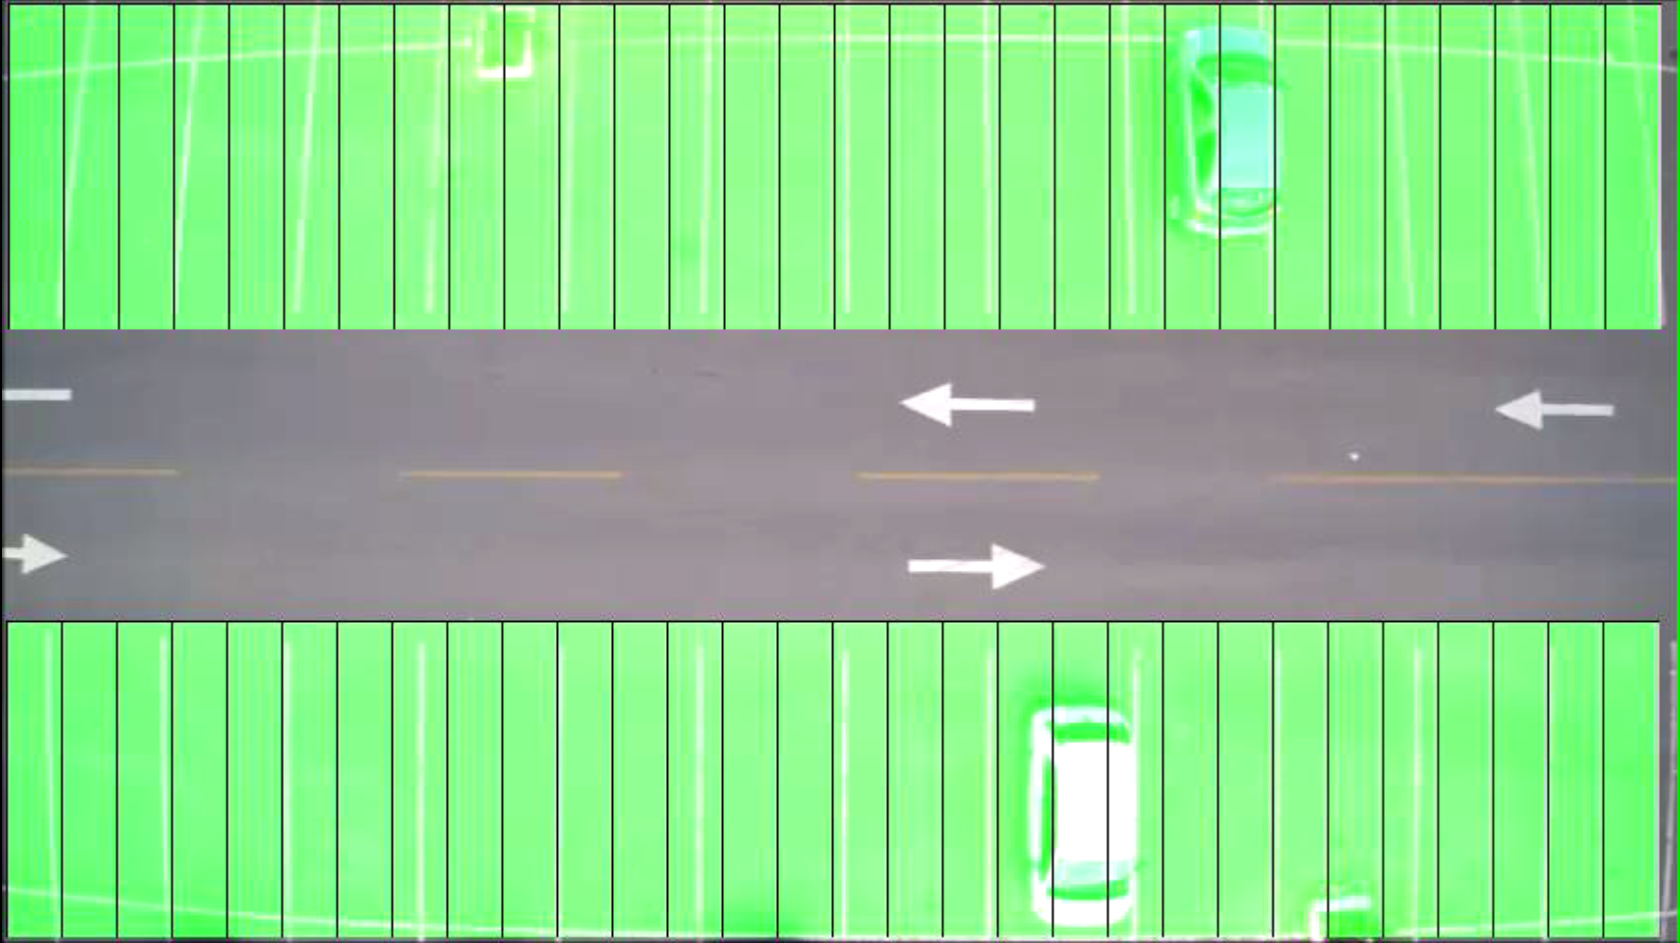
\includegraphics[width=.5\linewidth]{Video3Inicio}
\end{subfigure}\
\begin{subfigure}{.5\textwidth}
\centering
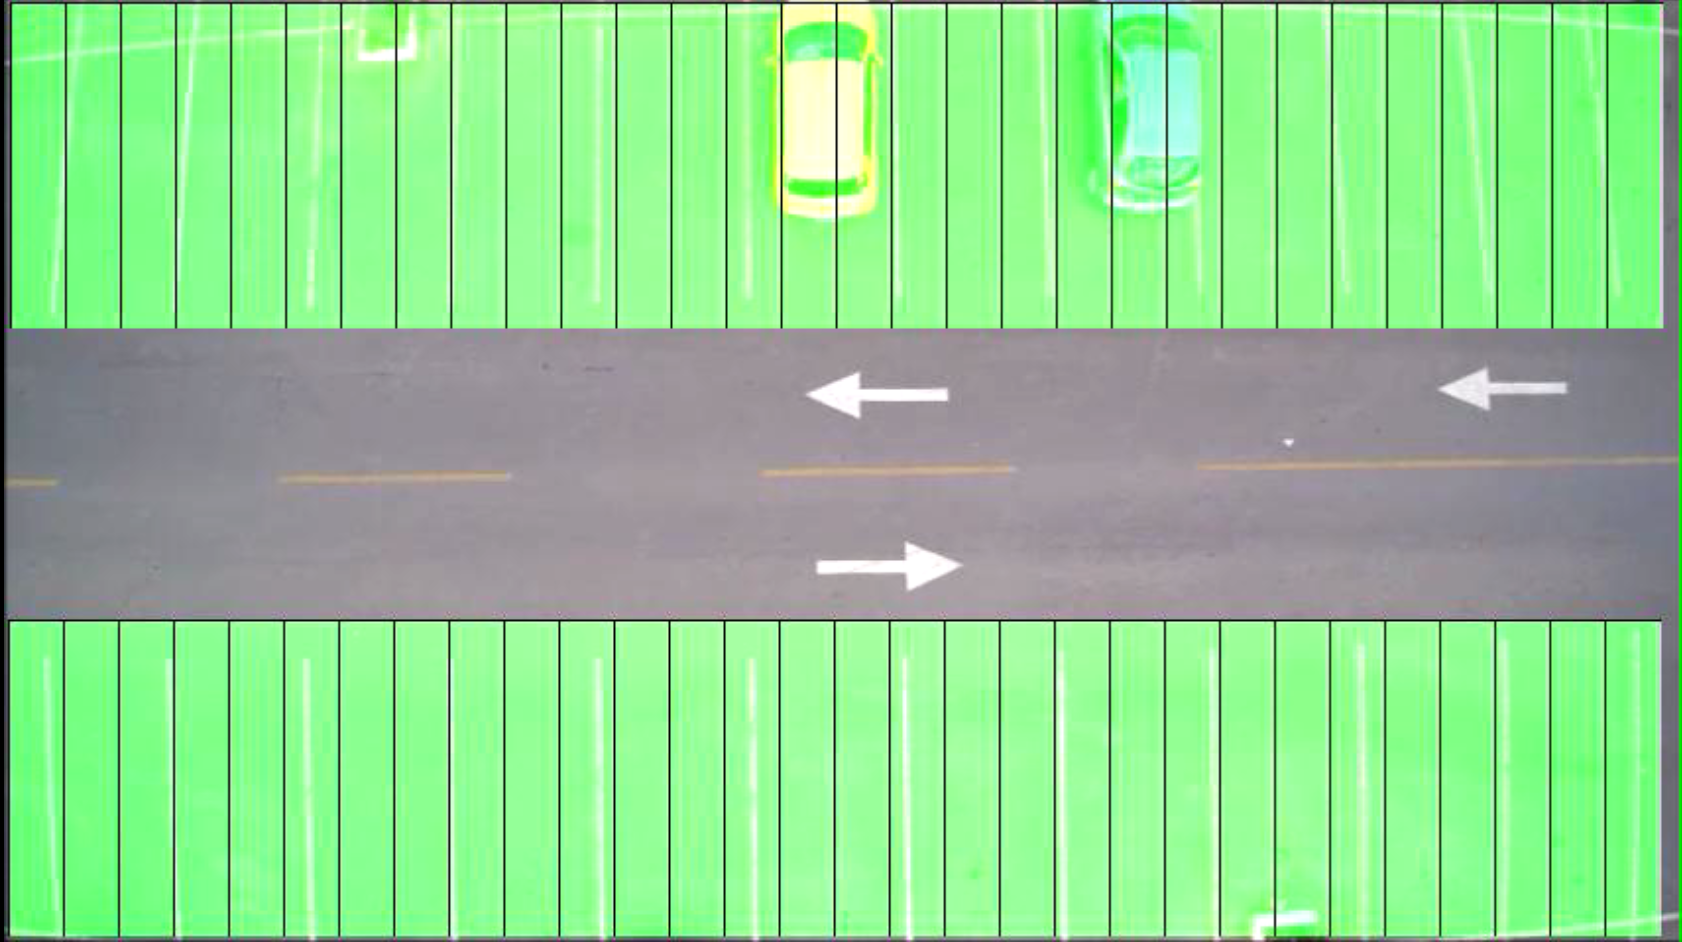
\includegraphics[width=.5\linewidth]{Video3Fim}
\end{subfigure}
\centering
\end{figure}	
\end{frame}

\begin{frame}
	\frametitle{Vídeo 3}
\begin{center}
\begin{tabular}{|c||c||c|}
\hline
Observador & Acertos & Taxa de acertos \\ \hline
F & 1165 & 97,08\% \\  \hline
P & 1113 & 92,75\% \\ \hline
M & 1136 & 94,66\% \\ \hline
Média & 1138 & 94,83\% \\
\hline
\end{tabular}
\end{center}
\end{frame}

\begin{frame}
\frametitle{Vídeo 3}
\begin{center}
\begin{tabular}{|c||c||c|}
\hline
\multicolumn{3}{|c|}{Acertos - vagas}  \\ \hline \hline
Observador & Acertos & Taxa de acertos \\ \hline
F & 19 & 95\% \\  \hline
P & 11 & 55\% \\ \hline
M & 18 & 90\% \\ \hline
Média & 16 & 80\% \\
\hline
\end{tabular}
\end{center}
\end{frame}


\begin{frame}
\frametitle{Vídeo 4}

Neste vídeo, o veículo branco entra em cena pela parte superior da tela e estaciona entre os outros dois carros. O carro cinza sai da vaga que ocupava e estaciona em uma na área inferior. Duração de $30s$.

\begin{figure}
\centering
\begin{subfigure}{.5\textwidth}
\centering
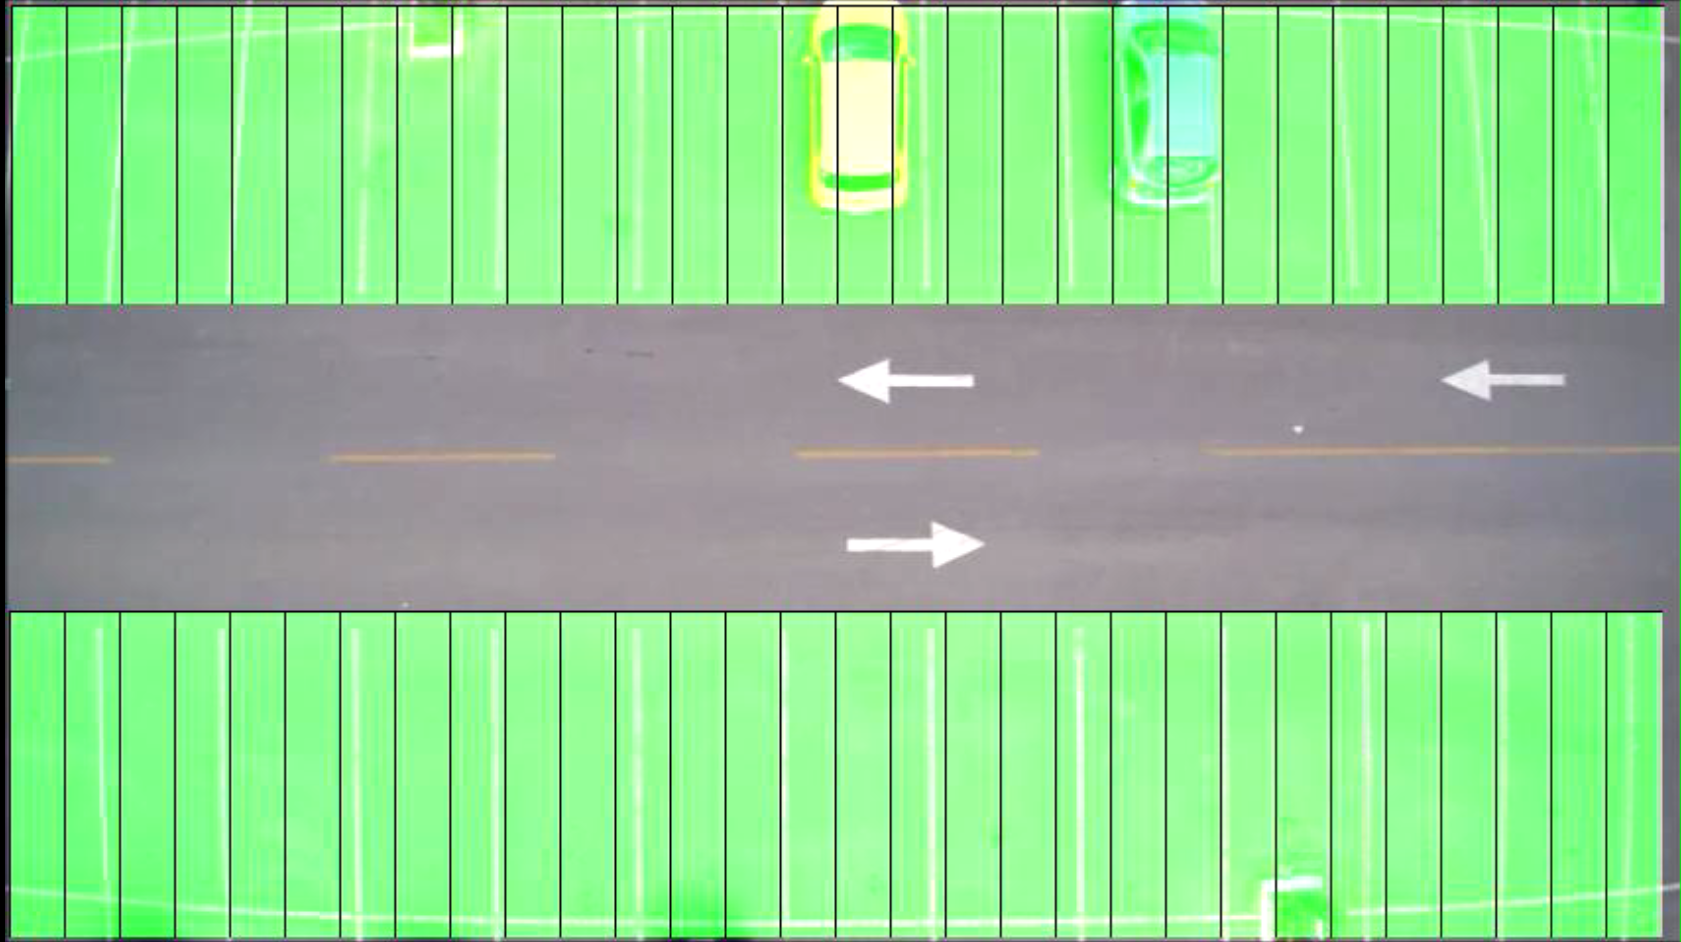
\includegraphics[width=.5\linewidth]{Video4Inicio}
\end{subfigure}\
\begin{subfigure}{.5\textwidth}
\centering
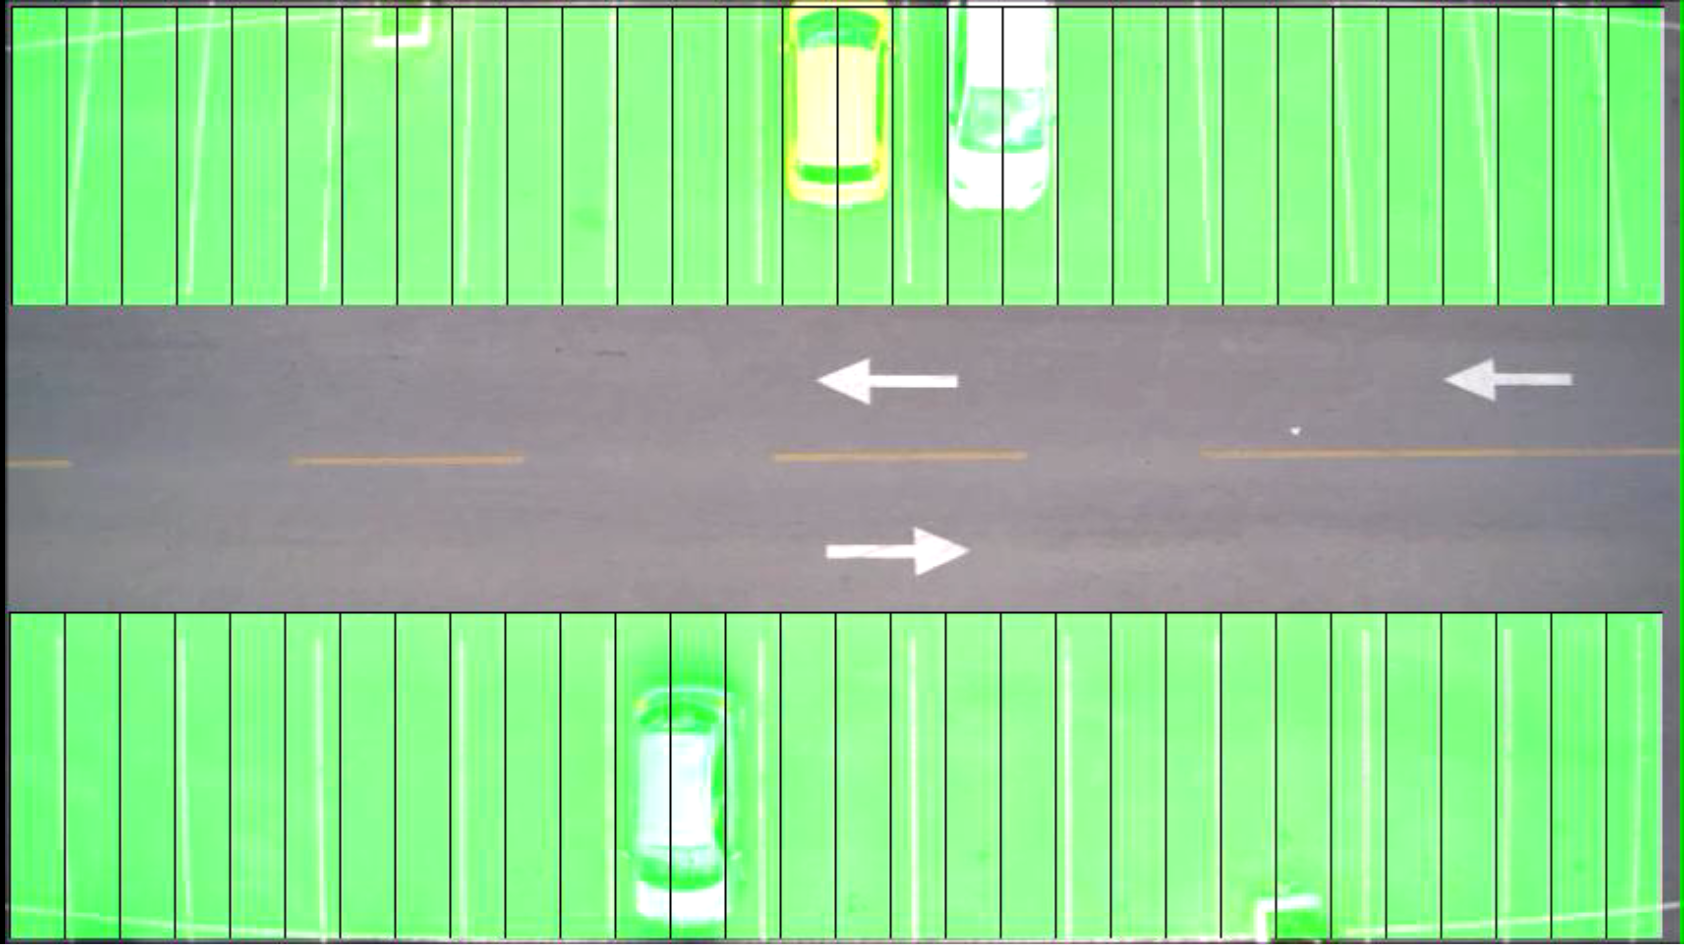
\includegraphics[width=.5\linewidth]{Video4Fim}
\end{subfigure}
\centering
\end{figure}	
\end{frame}

\begin{frame}
	\frametitle{Vídeo 4}
\begin{center}
\begin{tabular}{|c||c||c|}
\hline
\multicolumn{3}{|c|}{Acertos - seções}  \\ \hline \hline
Observador & Acertos & Taxa de acertos \\ \hline
F & 1750 & 97,22\% \\  \hline
P & 1749 & 97,16\% \\ \hline
M & 1772 & 98,44\% \\ \hline
Média & 1757 & 97,61\% \\
\hline
\end{tabular}
\end{center}
\end{frame}

\begin{frame}
\frametitle{Vídeo 4}
\begin{center}
\begin{tabular}{|c||c||c|}
\hline
\multicolumn{3}{|c|}{Acertos - vagas}  \\ \hline \hline
Observador & Acertos & Taxa de acertos \\ \hline
F & 22 & 73,33\% \\  \hline
P & 22 & 73,33\% \\ \hline
M & 24 & 80\% \\ \hline
Média & 22,66 & 75,55\% \\
\hline
\end{tabular}
\end{center}
\end{frame}

\begin{frame}
\frametitle{Vídeo 5}

Um veículo desocupa a sua vaga sainda pela parte superior da tela. Duração de $10s$.

\begin{figure}
\centering
\begin{subfigure}{.5\textwidth}
\centering
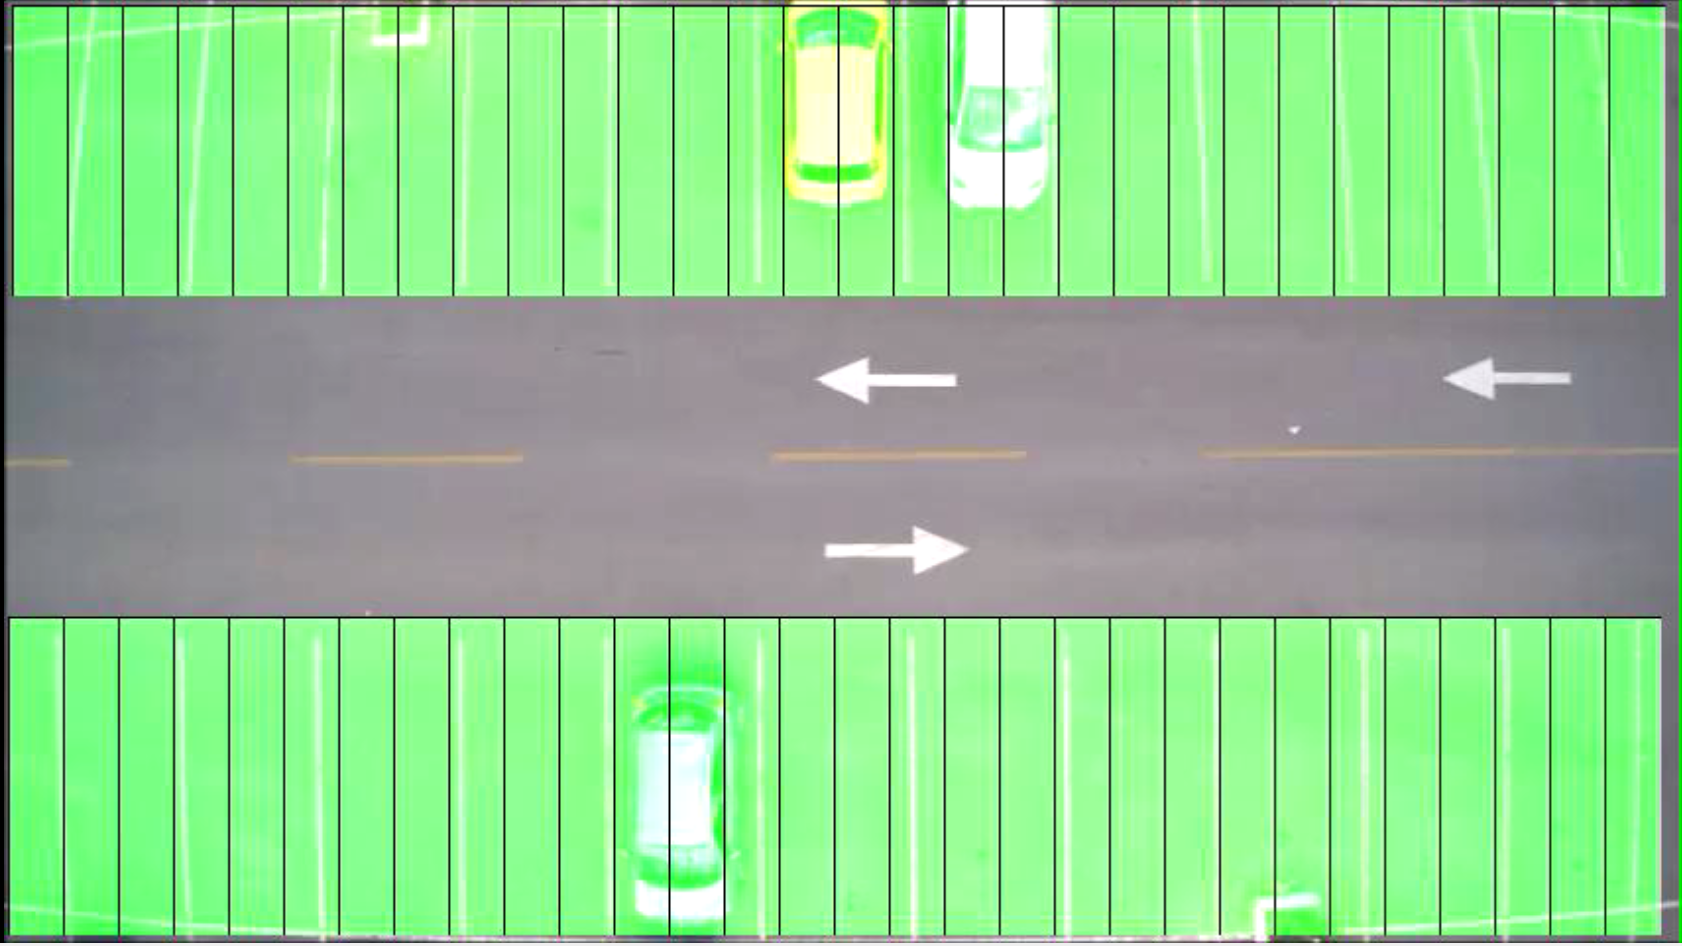
\includegraphics[width=.5\linewidth]{Video5Inicio}
\end{subfigure}\
\begin{subfigure}{.5\textwidth}
\centering
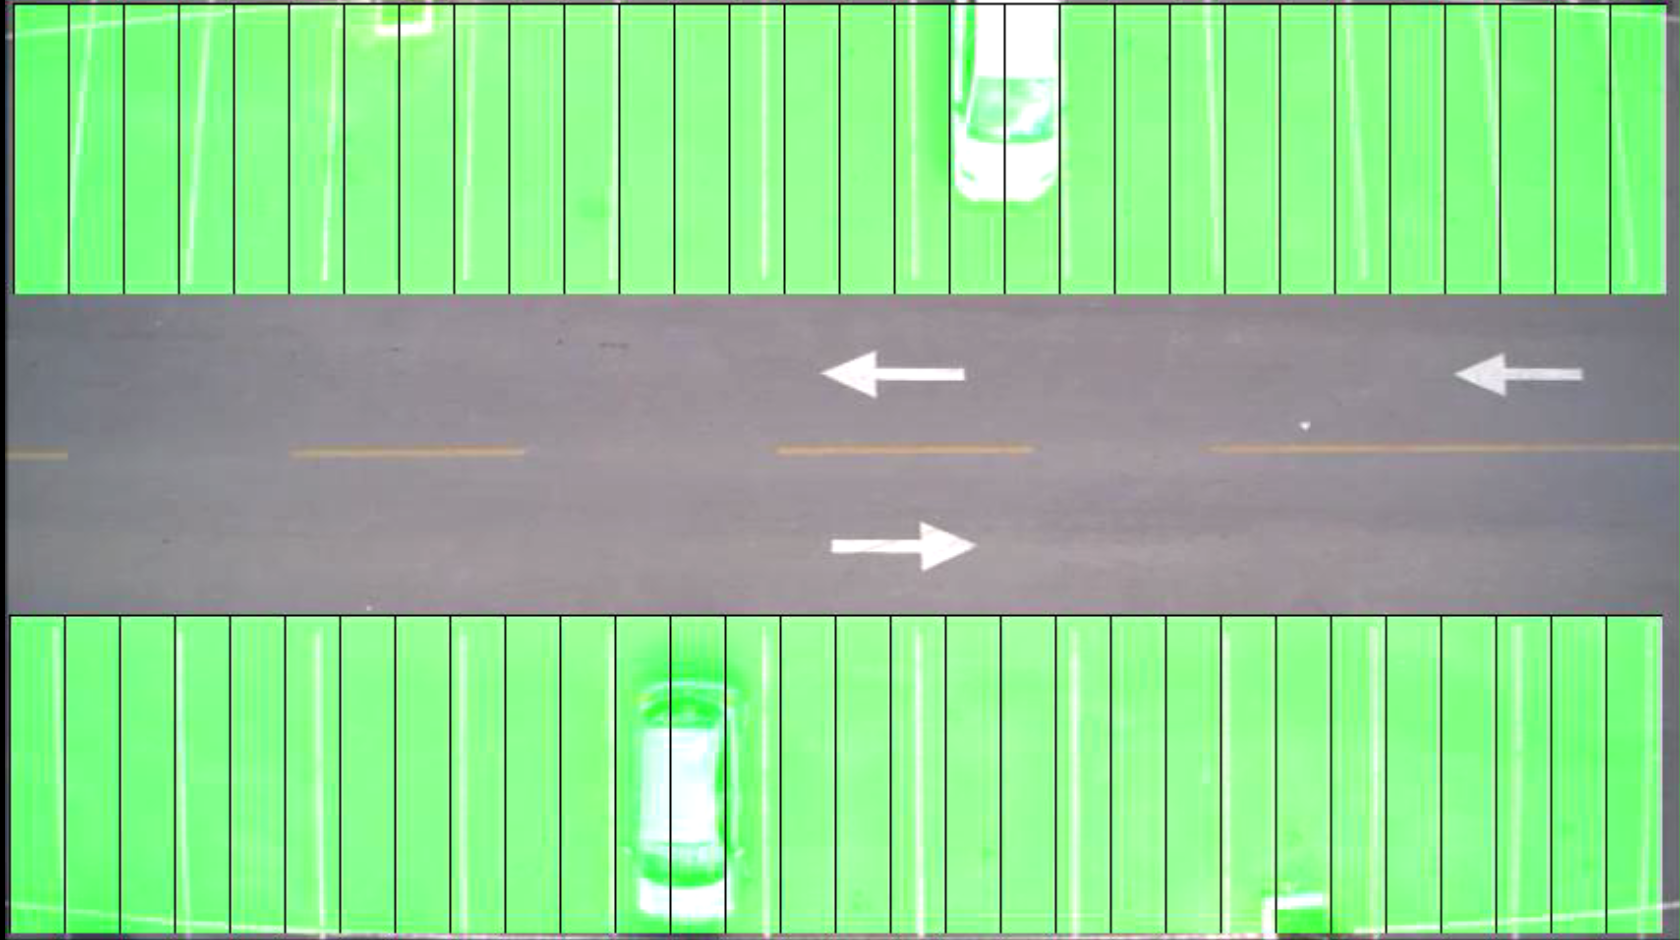
\includegraphics[width=.5\linewidth]{Video5Fim}
\end{subfigure}
\centering
\end{figure}	
\end{frame}

\begin{frame}
	\frametitle{Vídeo 5}
\begin{center}
\begin{tabular}{|c||c||c|}
\hline
\multicolumn{3}{|c|}{Acertos - seções}  \\ \hline
Observador & Acertos & Taxa de acertos \\ \hline
F & 597 & 99,50\% \\  \hline
P & 585 & 97,50\% \\ \hline
M & 587 & 97,83\% \\ \hline
Média & 1757 & 97,61\% \\
\hline
\end{tabular}
\end{center}
\end{frame}

\begin{frame}
\frametitle{Vídeo 5}
\begin{center}
\begin{tabular}{|c||c||c|}
\hline
\multicolumn{3}{|c|}{Acertos - vagas}  \\ \hline \hline
Observador & Acertos & Taxa de acertos \\ \hline
F & 10 & 100\% \\  \hline
P & 9 & 90\% \\ \hline
M & 10 & 100\% \\ \hline
Média & 9,66 & 9\% \\
\hline
\end{tabular}
\end{center}
\end{frame}

\begin{frame}
\frametitle{Vídeo 6}

Neste vídeo o veículo amarelo entra na cena pela parte inferior da tela. O veículo branco desocupa sua vaga e sai da tela pelo lado esquerdo. O vídeo tem $13s$.

\begin{figure}
\centering
\begin{subfigure}{.5\textwidth}
\centering
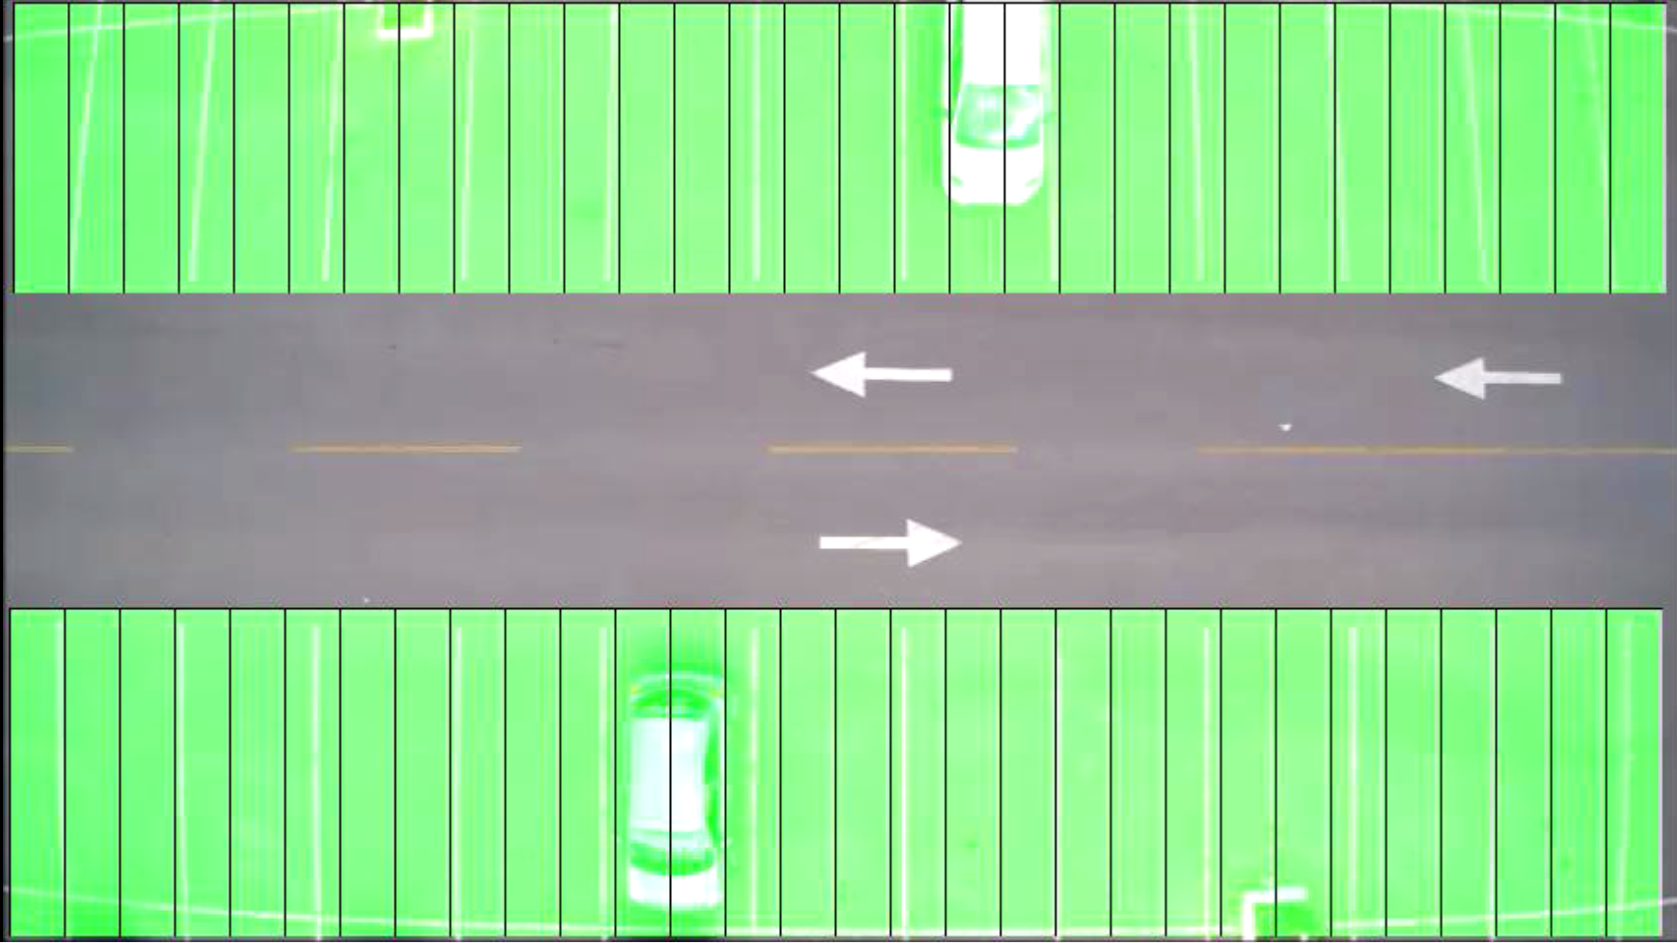
\includegraphics[width=.5\linewidth]{Video6Inicio}
\end{subfigure}\
\begin{subfigure}{.5\textwidth}
\centering
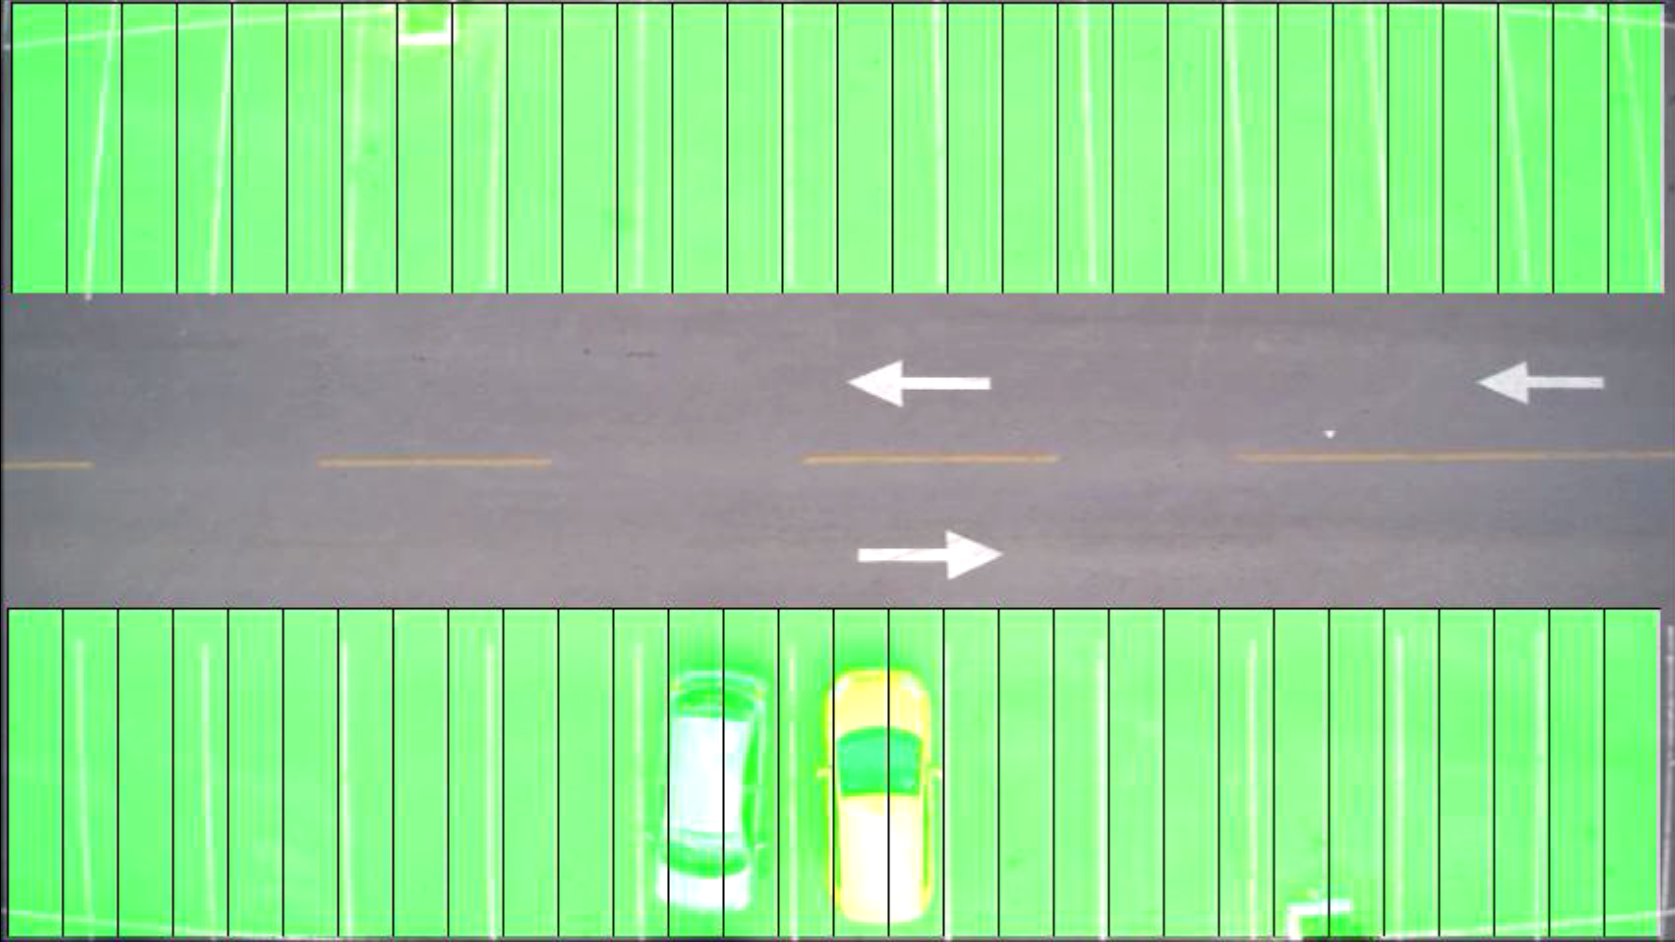
\includegraphics[width=.5\linewidth]{Video6Fim}
\end{subfigure}
\centering
\end{figure}	
\end{frame}

\begin{frame}
	\frametitle{Vídeo 6}
\begin{center}
\begin{tabular}{|c||c||c|}
\hline
\multicolumn{3}{|c|}{Acertos - seções}  \\ \hline
Observador & Acertos & Taxa de acertos \\ \hline
F & 752 & 96,40\% \\  \hline
P & 774 & 99,23\% \\ \hline
M & 767 & 98,33\% \\ \hline
Média & 764,33 & 97,99\% \\
\hline
\end{tabular}
\end{center}
\end{frame}

\begin{frame}
\frametitle{Vídeo 6}

\begin{center}
\begin{tabular}{|c||c||c|}
\hline
\multicolumn{3}{|c|}{Acertos - vagas}  \\ \hline \hline
Observador & Acertos & Taxa de acertos \\ \hline
F & 10 & 76,92\% \\  \hline
P & 11 & 84,61\% \\ \hline
M & 9 & 69,23\% \\ \hline
Média & 10 & 76,92\% \\
\hline
\end{tabular}
\end{center}
\end{frame}


\begin{frame}
\frametitle{Vídeo 7}
Neste vídeo um dos carros sai da cena pela esquerda. O vídeo tem $17s$.

\begin{figure}
\centering
\begin{subfigure}{.5\textwidth}
\centering
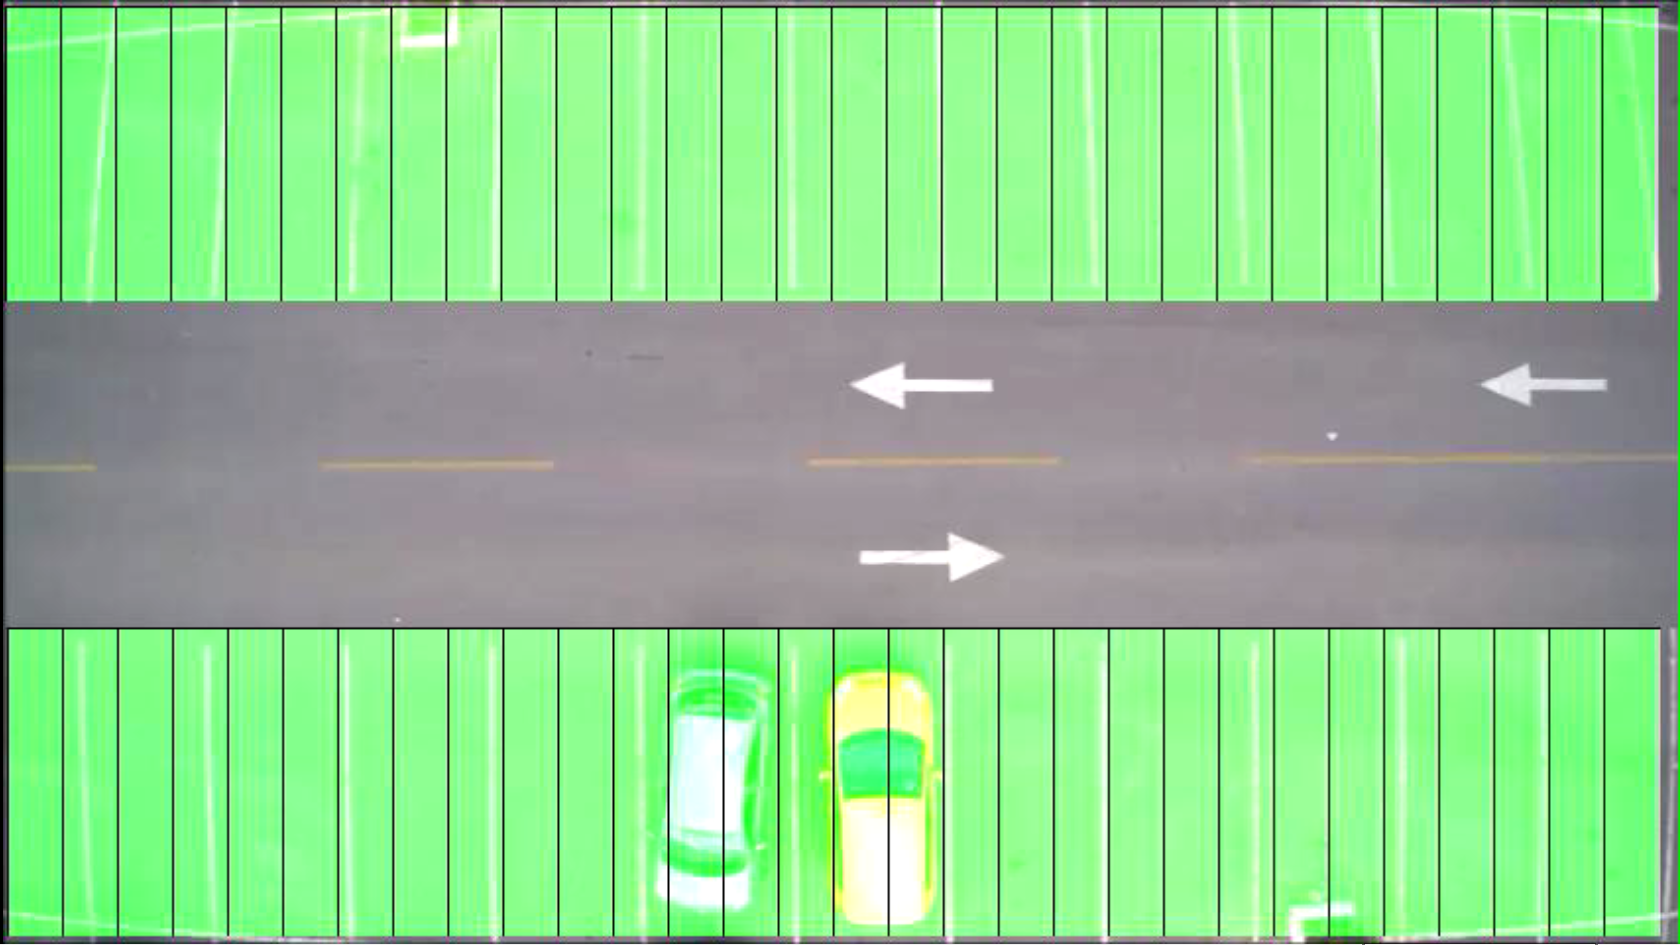
\includegraphics[width=.5\linewidth]{Video7Inicio}
\end{subfigure}\
\begin{subfigure}{.5\textwidth}
\centering
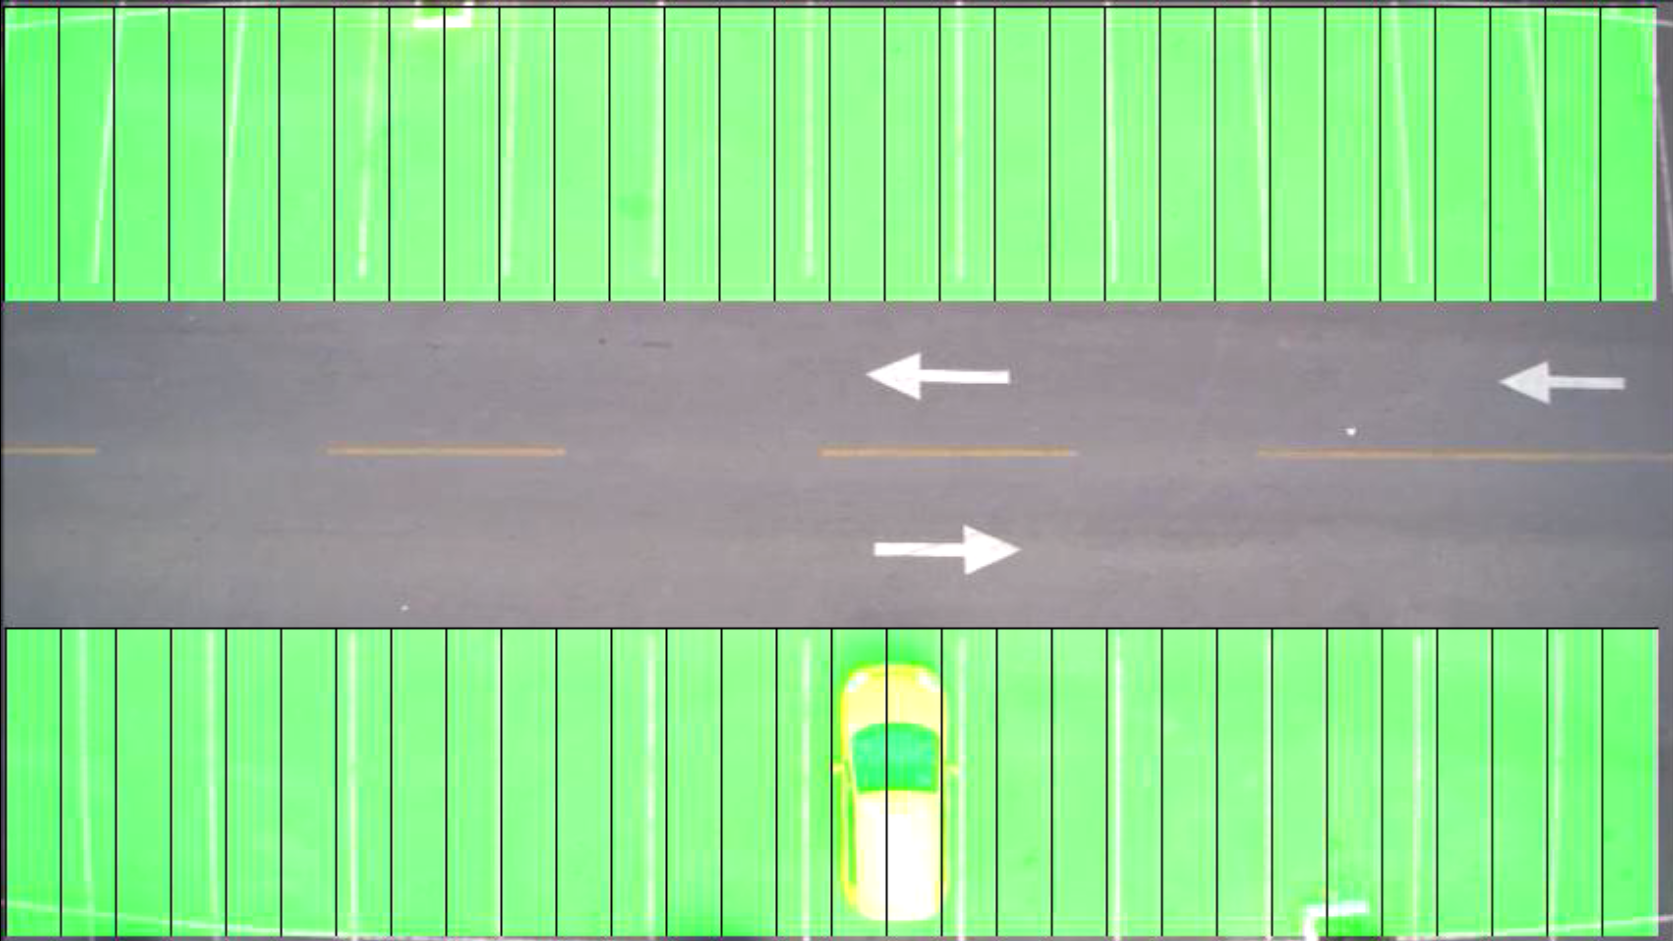
\includegraphics[width=.5\linewidth]{Video7Fim}
\end{subfigure}
\centering
\end{figure}	
\end{frame}

\begin{frame}
	\frametitle{Vídeo 7}
\begin{center}
\begin{tabular}{|c||c||c|}
\hline
\multicolumn{3}{|c|}{Acertos - seções}  \\ \hline
Observador & Acertos & Taxa de acertos \\ \hline
F & 1013 & 99,31\% \\  \hline
P & 1014 & 99,41\% \\ \hline
M & 1016 & 99,60\% \\ \hline
Média & 1014,33 & 99,44\% \\
\hline
\end{tabular}
\end{center}
\end{frame}

\begin{frame}
\frametitle{Vídeo 7}

\begin{center}
\begin{tabular}{|c||c||c|}
\hline
\multicolumn{3}{|c|}{Acertos - vagas}  \\ \hline \hline
Observador & Acertos & Taxa de acertos \\ \hline
F & 16 & 94,11\% \\  \hline
P & 16 & 94,11\% \\ \hline
M & 17 & 100\% \\ \hline
Média & 16,33 & 96,07\% \\
\hline
\end{tabular}
\end{center}
\end{frame}

\begin{frame}
\frametitle{Vídeo 7}
No oitavo e último caso de testes, um carro branco passa pela região central da imagem sem estacionar em nenhuma vaga e depois um carro cinza estaciona na região inferior. O vídeo tem $23s$ de duração.

\begin{figure}
\centering
\begin{subfigure}{.5\textwidth}
\centering
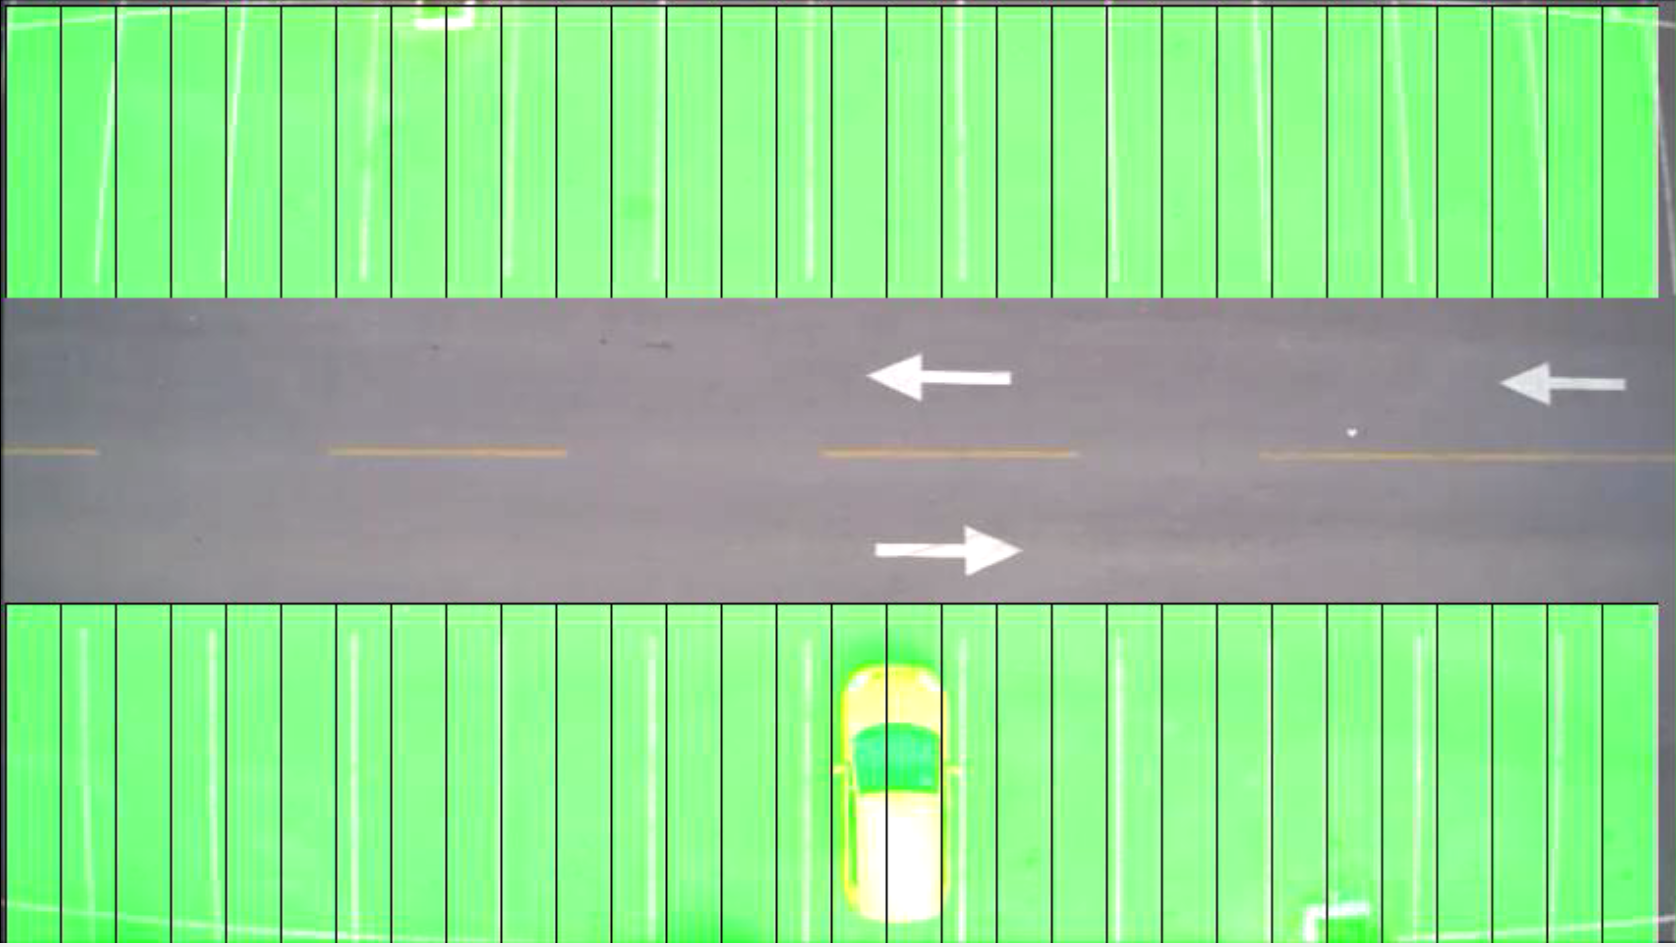
\includegraphics[width=.5\linewidth]{Video8Inicio}
\end{subfigure}\
\begin{subfigure}{.5\textwidth}
\centering
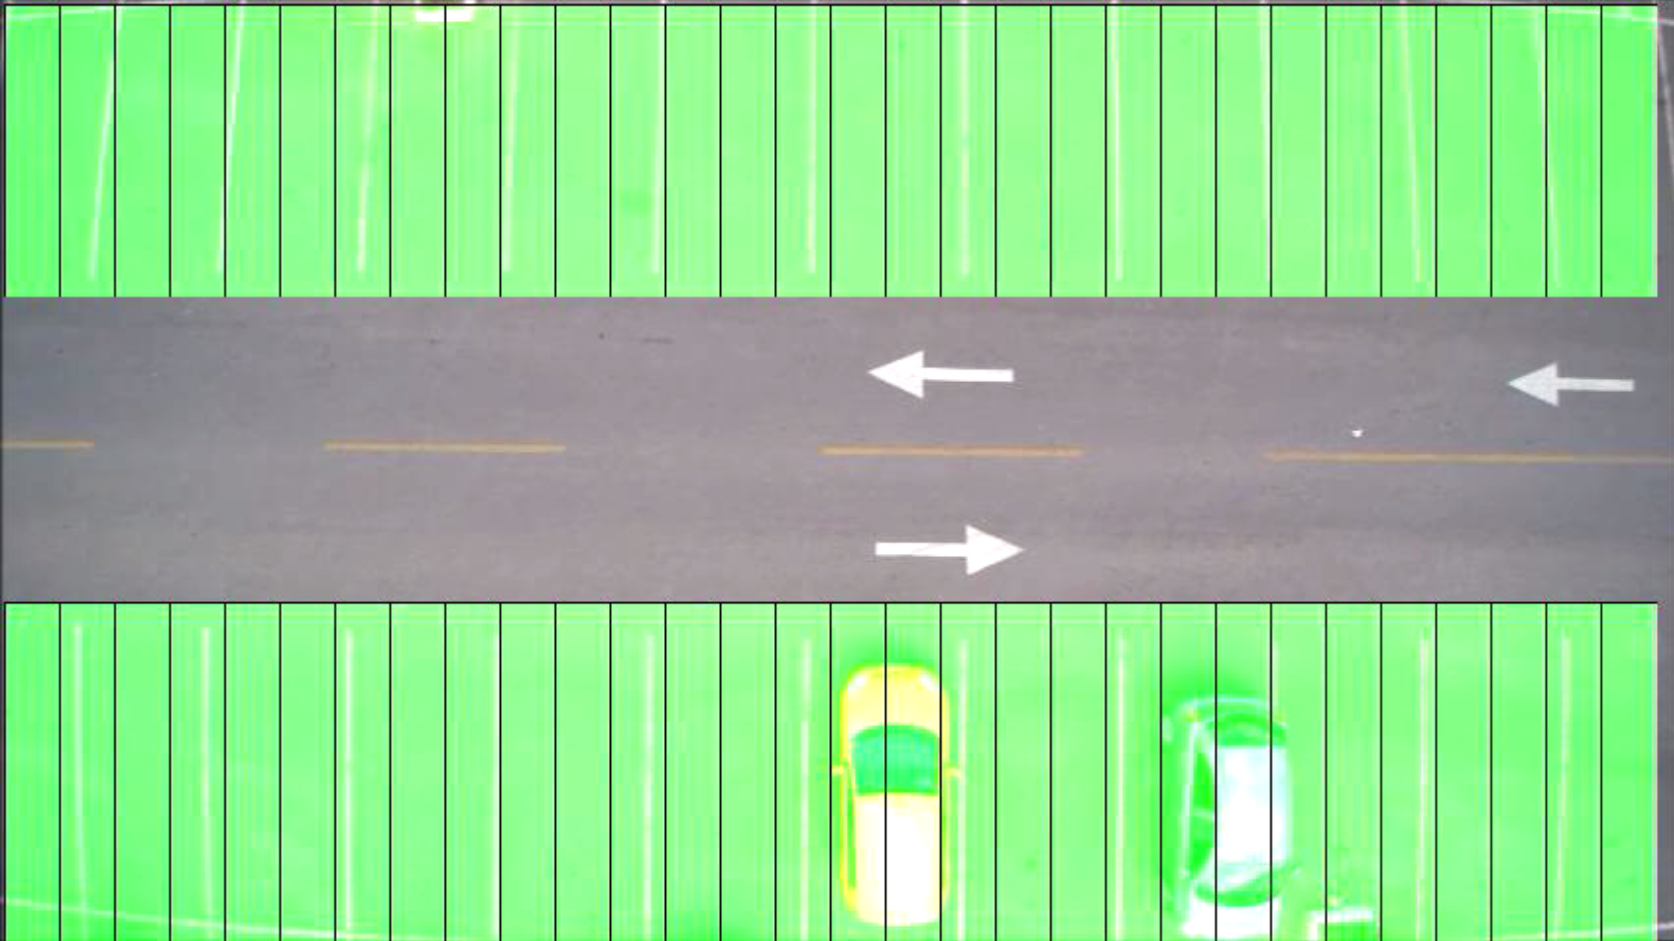
\includegraphics[width=.5\linewidth]{Video8Fim}
\end{subfigure}
\centering
\end{figure}	
\end{frame}

\begin{frame}
	\frametitle{Vídeo 8}
\begin{center}
\begin{tabular}{|c||c||c|}
\hline
\multicolumn{3}{|c|}{Acertos - seções}  \\ \hline\hline
Observador & Acertos & Taxa de acertos \\ \hline
F & 1376 & 99,71\% \\  \hline
P & 1379 & 99,92\% \\ \hline
M & 1379 & 99,92\% \\ \hline
Média & 1378 & 99,85\% \\
\hline
\end{tabular}
\end{center}
\end{frame}

\begin{frame}
\frametitle{Vídeo 8}

\begin{center}
\begin{tabular}{|c||c||c|}
\hline
\multicolumn{3}{|c|}{Acertos - vagas}  \\ \hline \hline
Observador & Acertos & Taxa de acertos \\ \hline
F & 23 & 100\% \\  \hline
P & 23 & 100\% \\ \hline
M & 23 & 100\% \\ \hline
Média & 23 & 100\% \\
\hline
\end{tabular}
\end{center}
\end{frame}




\section{Conclusao}
\begin{frame}
\frametitle{Conclusao}
\huge
Perguntas?

\end{frame}


\begin{frame}[allowframebreaks]
\frametitle{Referencias}
\bibliographystyle{plain}
\bibliography{bibliografia}

\end{frame}




\begin{frame}
\frametitle{Conclusao}
\huge
\cite{bong2008integrated} \cite{chen2012dynamic} \cite{de2006introduccao} \cite{delibaltov2013parking}\cite{gonzalez2009digital}
\cite{graciano2007rastreamento} \cite{hai2009self} \cite{IBGE2000introducao} \cite{idris09} \cite{marques1999processamento}
\cite{true2007vacant} \cite{vkl1989jain}
\end{frame}


%------------------------------%


\end{document} 